\documentclass{article}
\usepackage[utf8]{inputenc}
\usepackage{amsmath}
\usepackage{amsfonts}
\usepackage{graphicx}
\usepackage{mathtools}
\usepackage{commath}
\usepackage{float}
\DeclareUnicodeCharacter{00A0}{ }

\usepackage{xspace} % needed for \eg, \ie, \etc
\newcommand{\etal}[0]{{\em et~al.\@}\xspace}
\newcommand{\eg}[0]{{e.g.\@}\xspace}
\newcommand{\ie}[0]{{i.e.\@}\xspace}
\newcommand{\viz}[0]{{viz.\@}\xspace}
\newcommand{\resp}[0]{{resp.\@}\xspace}


\usepackage[english]{babel}
\usepackage{amsthm}
\theoremstyle{definition}
\newtheorem{definition}{Definition}[section]
\newtheorem{theorem}{Theorem}
\usepackage[linesnumbered,ruled]{algorithm2e}
\SetKwInOut{Parameter}{parameter}

\usepackage{graphicx}
\usepackage[caption=false]{subfig}
\usepackage{lipsum}

\addtolength{\oddsidemargin}{-.875in}
\addtolength{\evensidemargin}{-.875in}
\addtolength{\textwidth}{0.875in}

\addtolength{\topmargin}{-.875in}
\addtolength{\textheight}{1.75in}
\date{}


\begin{document}
\title{A Matrix-free Algorithm for PDE-governed Optimization with Inequality Constraints}
\author{
  Meng, Pengfei\\
  \and
  Dener, Alp\\
  \and 
  Hicken, Jason
}
\maketitle
\begin{abstract}
We present a matrix-free method for Partial-Differential-Equation(PDE) constrained optimization problems formulated in the reduced space. When many state-based constraints are present in the reduced-space formulation, it may not be practical to compute the constraint Jacobian explicitly.  This leads many practitioners to use constraint aggregation, which can produce overly conservative results.  A matrix-free Newton-Krylov optimization algorithm avoids these problems, but presents additional challenges related to globalization, preconditioning, and inequality constraint handling abilities. To address the former challenges, the proposed method uses a globally convergent homotopy continuation approach that uses a predictor-corrector algorithm to trace the solution curve. The predictor and corrector phases are solved using a Krylov iterative method that uses second-order adjoints to evaluate the necessary matrix-vector products. To cope with the poorly conditioned primal-dual system, a matrix-free preconditioner is proposed that uses a low-rank SVD approximation of the condensed Hessian term,  which is constructed using a certain number iterations of the Lanczos method. The algorithm is verified using analytical problems and exercised on a complex stress-constrained mass-minimization problem.  The method shows promising performance relative to a state-of-the-art matrix-based active-set algorithm, particularly for large numbers of design variables.
\end{abstract}

\section{Introduction}
We are interested in solving engineering design optimization problems that are governed by partial differential equations (PDEs). Such PDE-constrained optimization problems arise in many engineering applications including aerodynamic shape optimization \cite{lambe:2014,lyu2014aerodynamic, Zhang567303}, structural optimization \cite{DBLP:DeckelnickHJ17, lambe:2014, kennedy14}, and thermodynamic optimization \cite{chen1999finite,bejan2000thermodynamic,bejan2012thermodynamic}. A generic PDE-constrained optimization problem can be stated as
\begin{equation}\label{eq:gen1}
\begin{aligned}
\underset{x,u}{\text{min}} \quad &f(x, u) &\\
\text{subject to} \quad &  h(x,u) &= 0  \\
 &  g(x,u) &\geq 0  \\
 &  \mathcal{F}(x, u) &= 0, \\
\end{aligned}
\end{equation}
where $x \in \mathbb{R}^n, u \in \mathbb{R}^v$ are the design and state vectors respectively, and $f: \mathbb{R}^n \rightarrow \mathbb{R}, h: \mathbb{R}^n \rightarrow \mathbb{R}^l, g:\mathbb{R}^n \rightarrow \mathbb{R}^m$ are the objective, equality and inequality constraints respectively. We assume that $f$, $h$ and $g$ have continuous second derivatives. 

The challenge in solving \eqref{eq:gen1} is that general-purpose gradient-based optimization algorithms \cite{Nocedal2006NO, Byrd:1999:IPA:588897.589167,gill:2002} require the total derivative of the objective and constraints with respect to the design variables, and each of these total derivatives requires the solution of an $v\times v$ linear system, \ie a discretized PDE.  For example, the total derivative of the $i$th constraint $g_i$ is given by
\begin{align}
\frac{d}{dx}\left(g_i\right) &= \frac{\partial}{\partial x}\left(g_i\right) + \psi ^T \left[ \frac{\partial}{\partial x}\mathcal{F} \right] \\
\intertext{where $\psi \in \mathbb{R}^v$ is the adjoint which is governed by the discretized PDE,}
\left[ \frac{\partial}{\partial u}\mathcal{F} \right]^T \psi &= - \frac{\partial}{\partial u}\left(g_i\right) 
\end{align}
which is the adjoint equation \cite{Jameson03aerodynamicshape}. The computational cost of solving the adjoint equation is equivalent to that of the PDEs governing equation. Clearly, if the number of constraints $m$ is sufficiently large, it will be prohibitively expensive to compute all the total derivatives for optimization as each one entails an adjoint. 

To solve \eqref{eq:gen1}, the Lagrangian formulation is:
\begin{equation}\label{eq:lag}
\mathcal{L}(x, u, \psi, s, \lambda_h, \lambda_g) = f(x,u) + \lambda_h^T h(x, u) + \lambda_g^T (g(x,u)-s) + \psi^T \mathcal{F}(x,u),
\end{equation} 
where $s \in \mathbb{R}^m$ is for transforming the inequality constraints into equality ones, and $\lambda_h \in  \mathbb{R}^l$,  $\lambda_g \in  \mathbb{R}^m$ are the Lagrangian multiplier vectors for equality and inequality constraints. 

The first-order optimality conditions, or the \textit{Karush-Kuhn-Tucker} (KKT) conditions for \eqref{eq:gen1} are derived by taking partial derivatives of 
\eqref{eq:lag} with respect to all the unknown variables,
\begin{equation}\label{eq:kktcond}
\begin{aligned}
\nabla_x \mathcal{L} &= \nabla_x f + \lambda_h^T \nabla_x h + \lambda_g^T \nabla_x g + \psi^T \nabla_x\mathcal{F} = 0, \\
\nabla_u \mathcal{L} &= \nabla_u f + \lambda_h^T \nabla_u h + \lambda_g^T \nabla_u g + \psi^T \nabla_u\mathcal{F} = 0, \\
\nabla_{\psi} \mathcal{L} &= \mathcal{F} = 0, \\
\nabla_{\lambda_h} \mathcal{L} &= h = 0, \\
\nabla_{\lambda_g} \mathcal{L} &= g - s = 0, \\
-\mathcal{S} \Lambda_g e &= 0,\\
s \geq 0, &\quad \lambda_g \leq 0. \\
\end{aligned}
\end{equation}

The big nonlinear systems of equations \eqref{eq:kktcond} can be solved in either the full space or the reduced space.  Full-space methods~\cite{DBLP:journals/siamsc/BirosG05,DBLP:journals/siamsc/BirosG05a,haber:2001} solve all the unknowns in \eqref{eq:kktcond} simultaneously. The resulted KKT system is large, more than two times the number of state variables, indefinite and ill-conditioned. During optimization iterations, the state equation $\mathcal{F} =0$ and adjoint equation $\nabla_u \mathcal{L} = 0$ do not need to be solved exactly, avoiding the computational expense of tightly converging the PDE and adjoint equation residuals; however, this is also a potential disadvantage in practical engineering problems, because, if the optimization fails to converge, the intermediate solution may not be feasible with respect to the physics.  Furthermore, for highly nonlinear PDEs, \eg gas dynamics with shocks and boundary layers, practitioners have developed specialized globalization strategies that may be difficult to take advantage of in general-purpose full-space optimization algorithms.

In contrast, reduced-space algorithms treat the states $u$ and the adjoints $\psi$ as implicit functions of the design variables through $\mathcal{F}(x,u(x)) = 0$, $\nabla_u \mathcal{L} = 0$. The reduced KKT condition is formulated as follows, 
\begin{equation}\label{eq:opt00x}
\begin{aligned}
\nabla_x f + \lambda_h^T \nabla_x h + \lambda_g^T \nabla_x g &= 0, \\
-\mathcal{S} \Lambda_g e &= 0,\\
h &= 0, \\
g - s &= 0, \\
s \geq 0, \quad &\lambda_g \leq 0. \\
\end{aligned}
\end{equation}

Therefore, the resulted KKT system is much smaller, and it can make use of existing PDE solvers and adjoint solvers. Reduced-space methods have been successfully implemented in unconstrained problems and IDF problems. The unconstrained version of \eqref{eq:opt00x} can be solved efficiently using a Newton-Krylov (NK) algorithm applied to the first-order optimality conditions; see, for example, \cite{akcelik:2006, Heinkenschloss:1999:IOA, hinze2010optimization,borzi:2011}. NK optimization algorithms have also shown promise for equality-constrained optimization in the reduced space, because they do not require the constraint Jacobian to be form explicitly and, thus, avoid the scaling issue described earlier.  For instance, \cite{dener:idf2017} applied a matrix-free NK algorithm to a class of equality-constrained optimization problems that arise in multidisciplinary design optimization and would otherwise be intractable with conventional matrix-based algorithms.

Motivated by its success in the unconstrained and equality-constrained cases, we would like to extend the NK methodology to  more general, inequality constrained problems, to solve \eqref{eq:opt00x} using Newton Krylov methods. 

%\begin{equation}\label{eq:redform}
%\begin{aligned}
%&\text{min}   &f(x, u(x)) &\\
%&\text{s.t.} & h(x,u(x)) &= 0   \\
%& &  g(x,u(x)) &\geq 0 \\
%\end{aligned}
%\end{equation}

However, while NK methods can avoid the cost associated with forming the explicit constraint Jacobian, this extension faces several significant challenges. First, active-set and interior-point algorithms that make use of an explicit basis for the null space of the constraint Jacobian cannot be used, because such a basis requires the Jacobian to be explicitly available.  Second, the primal-dual saddle-point system raised in optimization is indefinite and ill-conditioned, making it difficult for iterative Krylov methods to converge to a sufficient tolerance, hurting the convergence rate of Newton's method. Third, dealing with nonconvex Hessian of the Lagrangian in the null space of the constraint Jacobian is also a non-trivial task. 

% Although the simulation problem is usually well-posed, the optimization problem is indefinite and ill-conditioned, which, combined with the large size of modern engineering problems and the expensive cost of PDE solve and adjoint solve, makes PDE-constrained optimization a significant challenge for general-purpose optimization algorithms. 
% Researchers have been investigating special-purpose optimization algorithms for PDE-constrained optimization problems. One major alternative is Full-Space Newton-Krylov method \cite{DBLP:journals/siamsc/BirosG05,DBLP:journals/siamsc/BirosG05a,haber:2001} that solves for the design, state and adjoint vectors simultaneously using a Krylov method at each Newton step. But the system matrix is usually indefinite, ill-conditioned and huge. 

% In contrast, Reduced-Space Newton-Krylov method \cite{akcelik:2006} treats state and adjoint vectors as implicit functions of the design variables, thus it is possible to capitalize on existing PDE and adjoint solvers. The reduced-space optimization problem is formulated as
% Globalization strategies is difficult to find as the system features are highly problem-dependent, thus greater intrusions into the solvers are needed.

% For instance, to ensure progress towards global minimum, either trust-region or line-search globalization techniques have to be implemented. The former judges the quality of a computed step by calculating the merit function value and adjust the trust-region radius accordingly, while the latter computes the step-length along a step direction that satisfies the Wolfe condition. In either case, extra computation is needed. Dealing with nonconvex Hessian of the Lagrangian in the null space of the constraint Jacobian is also a non-trivial task; possible solutions include adding a proper regularization term to enforce a positive definite Hessian, see \cite{hicken:flecs2014} and Algorithm B.1 \cite{Nocedal2006NO}. Moreover, the saddle-point matrix raised in optimization is indefinite and ill-conditioned, making it difficult for iterative Krylov methods to converge. 

Homotopy methods are robust, numerically stable, and globally convergent, see \cite{allgower_georg_1993}, \cite{Watson_1989}. They have been successfully applied to difficult nonlinear PDEs, see \cite{hicken:cfd2009, hicken:cfd2011b}, and \cite{Brown_2016}.  In optimization, globally convergent probability-one homotopy methods have been successfully applied on engineering optimization problems. \cite{Watson_2001} developed general convergence theory for nonlinear inequality constrained optimization, from unconstrained, bound-constrained, linear and nonlinear inequality constrained convex cases to nonconvex cases. The complementarity conditions are replaced by a cubic nonlinear system involving the multipliers and constraints. However, equality constraints are not covered, and it is not straightforward to implement it using Newton-Krylov methods. Huang et al. \cite{huang_2012pc} transfered a general nonlinear optimization with equality and inequality into an inequality only problem, and used the predictor-corrector method to track the homotopy interior point map using the Conjugate Gradient method. The method derived and achieved global linear convergence under the normal cone condition. However it does not handle nonconvex objective and constraint functions. 

To address the challenges, we propose using homotopy continuation methods to solve the reduced KKT condition \eqref{eq:opt00x} from reduced-space PDE-constrained optimization problems, which comes with a natural regularization term that functions like a globalization unit and improves the condition and convexity of the system. Alongside the iterative Krylov solver used in the homotopy method, a matrix-free preconditioner based on SVD approximation is used to accelerate its convergence rate. 

The paper is organized as follows. In Section 2, the proposed homotopy-based globlization optimization method is explained in detail. Section 3 introduces matrix-free preconditioners accelerating the convergence of the Krylov method used in optimization. Section 4 includes three test problems to show the performance of the new method. First on a constructed nonconvex problem to see the nonconvexity handling ability of the new method; second on a linearly constrained quadratic problem with the Hessian of the objective and the constraint Jacobian have known SVD decompositions to verify the new method and the matrix-free preconditioner; and lastly on a practical PDE-constrained structural sizing design problem with the numerical experiment results benchmarked SNOPT, which is a popular active-set SQP optimization package. Section 5 is on conclusions and future work.      

\section{A Homotopy-based Globalization for PDE-Constrained Optimization}

\subsection{Homotopy map for optimization}
Conceptually, the idea of homotopy methods is simple. To find the solution of a function $\mathcal{R}(x)$, a homotopy map is constructed connecting the target function with an easy function through a weighting parameter. For example:
\begin{equation*}
\mathcal{H}_a\left(\mu, x\right) = (1-\mu) \mathcal{R}(x) + \mu g_a(x), \quad 0 \leq \mu \leq 1
\end{equation*}
where $g_a(x)$ is the simple function with obvious solutions, and $\mu$ is the homotopy parameter. 

We use a simple optimization example to illustrate the idea. To minimize the following cubic polynomial function within a certain interval, 
\begin{equation*}
\text{min}  \quad  f(x) = -\frac{x^3}{3} + \frac{x^2}{2},  \qquad  x \in [0, 1.0]\\
\end{equation*}

%The target in optimization is to find the solution of the first-order gradient function:
%\begin{equation*}
%f(x) = -x^2 + x,  \qquad  x \in [0, 1.5]\\
%\end{equation*}

A homotopy function is constructed based on the first-order gradient of the polynomial and an easy function, 
\begin{equation*}
\mathcal{H} \left(\mu, x\right) = (1-\mu) \nabla f(x) + \mu (x-a), \quad a \in [0, 1.0] \\
\end{equation*}
whose solution curves corresponding to different values of $a$ are shown in Fig. \ref{fig:zc} below,
\begin{figure}[H]
  \centering
  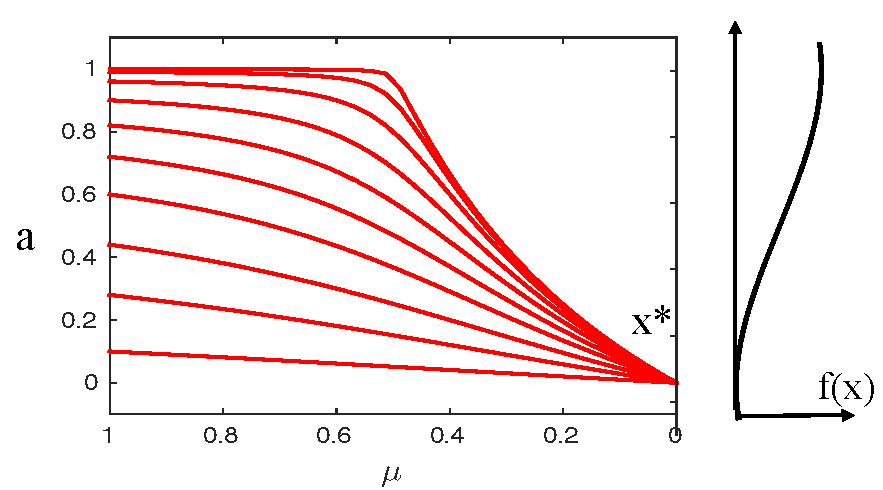
\includegraphics[width=0.7\textwidth]{./figs/zero_curve.pdf}
  \caption{Solution curves for $\mathcal{H}=0$ at different values of $a$}
  \label{fig:zc}
\end{figure}

For a certain value $a$, when $\mu$ changes from $1.0$ to $0.0$, the solution trajectory starts from the solution of the easy function and ends at the solution of the target function. Homotopy continuation method are usually applied on much more complex problems, \eg large-scale engineering problems. For such cases, the shape of the solution curves is much less intuitive and whether they are traceable needs proof. The Parametrized Sard's Theorem, which is from Definition 2.1 and Theorem 2.2 in \cite{watson_2002} and \cite{chow_1978} is restated here:

\theoremstyle{definition}
\begin{definition}
Let $U \subset \mathbb{R}^m$ and $V \subset \mathbb{R}^p $ be open sets, and let $\mathcal{H} : U \times (0,1] \times V \rightarrow \mathbb{R}^p $ be a $C^2$ map. $\mathcal{H}$ is said to be transversal to zero if the $p \times (m + 1 + p)$ Jacobian matrix $D\mathcal{H}$ has full rank on $\mathcal{H} ^{-1}(0)$.   
\end{definition}

\begin{theorem}[Parametrized Sard's Theorem]
Let $\mathcal{H} : U \times (0,1] \times V \rightarrow \mathbb{R}^p $ be a $C^2$ map. If $\mathcal{H}$ is transversal to zero, then for almost all $a \in U$ the map 
\begin{equation*}
\mathcal{H}_a(\lambda, x) = \mathcal{H}(a, \lambda, x) 
\end{equation*}
is also transversal to zero.
\end{theorem}

The theorem basically says that if there exists one homotopy map whose Jacobian matrix is nonsingular on its solution curve (the solution curve is smooth), then for almost all $a \in U$, the homotopy map $\mathcal{H}_a$ also has a nonsingular Jacobian on its solution curve. 

In optimization, we want to solve the first order necessary optimality condition: 
\begin{equation}
\mathcal{R}(\boldsymbol{q}) =\mathcal{R}(x,s,\lambda_h, \lambda_g) = \begin{bmatrix}
\nabla_x f(x)  + \lambda_h^T \nabla_x h(x)  + \lambda_g^T \nabla_x g(x)   \\
-\mathcal{S}\Lambda_g e\\
h(x) \\
g(x) - s 
\end{bmatrix} = 0.
\end{equation}

For the homotopy map, we use the linear function $g_a(x) = x - a$ as the homotopy term, and a linear convex combination between the target function and the easy function:
\begin{equation}\label{eq:homo0}
\begin{aligned}
\mathcal{H}(\boldsymbol{q}, \mu) &= (1-\mu) \mathcal{R}(\boldsymbol{q}) + \mu(\boldsymbol{q} - \boldsymbol{q}_0) \\ 
&= (1-\mu) \begin{bmatrix}
\nabla_x f(x)  + \lambda_h^T \nabla_x h(x)  + \lambda_g^T \nabla_x g(x)   \\
-\mathcal{S}\Lambda_g e \\
h(x) \\
g(x) - s 
\end{bmatrix}  + \mu 
\begin{bmatrix}
x-x_0 \\
s-s_0 \\
- (\lambda_h - \lambda_{h0} )  \\
- (\lambda_g - \lambda_{g0} ) 
\end{bmatrix}
\end{aligned}
\end{equation}
where $\boldsymbol{q} = [x, s, \lambda_{h}, \lambda_{g}]$ represents the KKT vector, and $\boldsymbol{q}_0$ is chosen as: $x_0$ any initial design point, $s_0$ the slacks corresponding to the inequality constraints, $\lambda_{h0}$ and $\lambda_{g0}$ are vectors of zeros.

In respect to the Theorem and Definition, the homotopy map in \eqref{eq:homo0} is a $C^2$ map. 
%Although we could not prove it theoretically for now, numerical evidence so far has confirm that the Jacobian of the homotopy map  $\partial \mathcal{H}/\partial \boldsymbol{q}$ is nonsingular on the solution curve. 

% the Jacobian of the homotopy map is nonsingular on the solution curve, 
% If the target function $f(x)$ is smooth and has a solution, then for almost every $a$, the zeros of the homotopy contains a smooth curve that leads from the zeros of $g_a$ to zeros of $f$, and the Jacobian of the homotopy map is nonsingular along its zero-curve. 

\subsection{Predictor-Corrector methods}
We use a predictor-corrector algorithm to trace the zero-curve of the homotopy map, see \cite{allgower_georg_1993} and its references. Fig. \ref{fig:pc} illustrates the predictor and corrector phases at a certain point on the path. At a predictor step, tangent direction is calculated, and the value of $\mu$ and $\boldsymbol{q}$ are updated simultaneously by moving along the tangent. At a corrector step, the value of $\mu$ is fixed, and the homotopy function is solved using inexact Newton method to bring the solution closer to the zero-curve path. The cycle is repeated until $\mu$ is equal to machine zero, and the solution of the primal-dual system is recovered.

\begin{figure}[H]
  \centering
  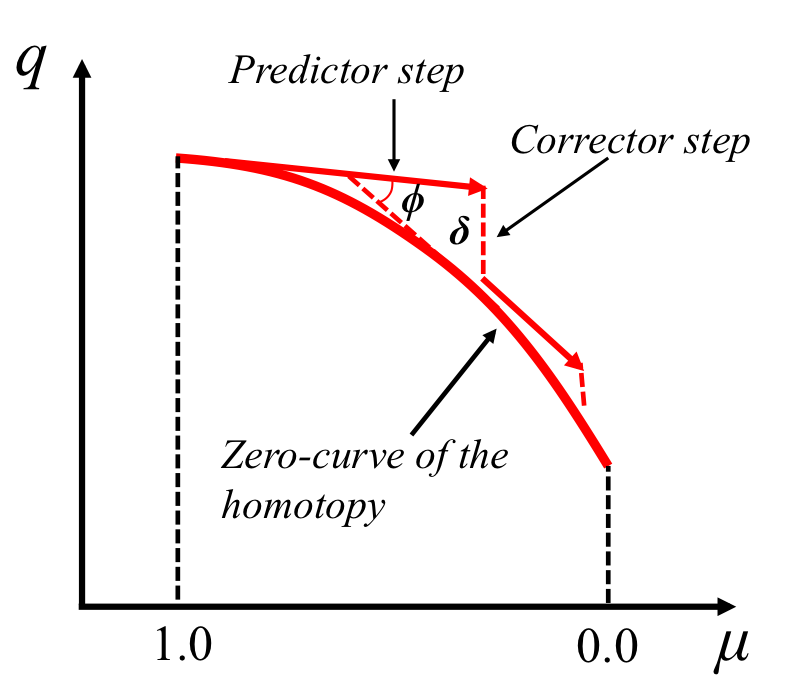
\includegraphics[width=0.5\textwidth]{./figs/PC_graph.png}
  \caption{Illustration of Predictor-Corrector Algorithm}
  \label{fig:pc}
\end{figure}

\subsubsection{Predictor}
During a predictor step we need the tangent direction $d\boldsymbol{q}/d\mu$, which can be found by taking the total derivative of $\mathcal{H}$ with respect to $\mu$:
\begin{align}\label{eq:pctan}
\ \ \qquad \mathcal{H}(\boldsymbol{q}(\mu), \mu) &= 0 \notag \\
\Rightarrow \qquad \frac{d \mathcal{H} }{d \mu} &= 
\frac{\partial \mathcal{H}}{\partial \boldsymbol{q}} \frac{d \boldsymbol{q} }{d \mu} + \frac{\partial \mathcal{H}}{\partial \mu} = 0  \notag \\
\Rightarrow \qquad \frac{d \boldsymbol{q} }{d \mu} &= - \left( \frac{\partial \mathcal{H}}{\partial \boldsymbol{q}}\right)^{-1} \frac{\partial \mathcal{H}}{\partial \mu}  
\end{align}

In practice, \eqref{eq:pctan} is the linear system to be solved to get $\frac{d \boldsymbol{q} }{d \mu} $, and to put it in another way: 
\begin{equation}\label{eq:predictorx}
\frac{\partial \mathcal{H}}{\partial \boldsymbol{q}} \left( \frac{d \boldsymbol{q} }{d \mu}\right) = -\frac{\partial \mathcal{H}}{\partial \mu}
\end{equation}

We use a preconditioned Krylov iterative method to solve \eqref{eq:predictorx} inexactly, which will be described in detail in Section 3. 

Next, the predictor direction should reflect the changes in both $\boldsymbol{q}$ and $\mu$, with $\mu$ decreasing along the solution curve. Therefore, the normalized tangent direction $\boldsymbol{t}$ given by 
\begin{equation}
\begin{aligned}
\boldsymbol{t} &= \frac{\boldsymbol{\tau}}{\lVert \boldsymbol{\tau}\rVert } \\
\boldsymbol{\tau} &= \begin{bmatrix}
-\frac{d \boldsymbol{q} }{d \mu} \\ -1 
\end{bmatrix} 
= \begin{bmatrix}
\left( \frac{\partial \mathcal{H}}{\partial \boldsymbol{q}}\right)^{-1} \frac{\partial \mathcal{H}}{\partial \mu} \\
-1 
\end{bmatrix} 
\end{aligned}
\end{equation}

Then the predictor step is updated according to:
\begin{equation}\label{eq:pred}
\begin{bmatrix}
\boldsymbol{q}_{k+1}' \\ \mu_{k+1} 
\end{bmatrix} 
=\begin{bmatrix}
\boldsymbol{q}_k \\ \mu_k 
\end{bmatrix} 
+ \alpha \boldsymbol{\tau}
\end{equation}
where $\alpha$ is the step length taken along the predictor direction and will be described shortly.  

\subsubsection{Corrector}
At a corrector phase, with $\mu$ fixed based on the previous predictor step update, an inexact-Newton method is applied to solve the homotopy equation such that the relative residual of the homotopy function is below some small tolerance
\begin{equation}\label{eq:cornt}
\frac{\lVert \mathcal{H}\left(\boldsymbol{q}_k^{(n)}, \mu_k \right) \rVert}{\lVert \mathcal{H}\left(\boldsymbol{q}_k^{(0)}, \mu_k \right) \rVert} \leq \epsilon_k \in [0.1, 0.5]
\end{equation}

The loose tolerance $\epsilon_k \in [0.1, 0.5]$ is for intermediate iterations before $\mu_k$ reaches zero. At the last corrector phase when $\mu_k = 0.0$, the tolerance is tightened so that the targeted optimality and feasibility are satisfactory.  

At each Newton step, the linear system to be solved is given by
\begin{equation}\label{eq:cor}
\frac{\partial \mathcal{H}}{\partial \boldsymbol{q}} \Delta \boldsymbol{q} = -\mathcal{H} 
\end{equation}

The system matrix used in a corrector phase and a predictor phase have the same formulations:
\begin{equation}\label{eq:dHdq}
\frac{\partial \mathcal{H}}{\partial \boldsymbol{q}} = (1-\mu)\begin{bmatrix}
 \nabla_{xx} \mathcal{L}   & \boldsymbol{0} & \mathcal{A}^T_h   & \mathcal{A}^T_g   \\
\boldsymbol{0}     &  - \Lambda_g \mathcal{S}   & \boldsymbol{0} & -\mathcal{S}     \\
\mathcal{A}_h  &  \boldsymbol{0}   & \boldsymbol{0} &  \boldsymbol{0}  \\
\mathcal{A}_g  & -\mathcal{S}  &  \boldsymbol{0}  & \boldsymbol{0}   \\
\end{bmatrix}
+ \mu \begin{bmatrix}
\mathcal{I} & \boldsymbol{0} & \boldsymbol{0} & \boldsymbol{0} \\
\boldsymbol{0}  & \mathcal{S}  & \boldsymbol{0} & \boldsymbol{0} \\
\boldsymbol{0} & \boldsymbol{0} & -\mathcal{I} &  \boldsymbol{0} \\
\boldsymbol{0} & \boldsymbol{0} &   \boldsymbol{0} & -\mathcal{I} 
\end{bmatrix}
\end{equation}

\subsubsection{Step-length $\alpha$}
Finally, the step-length $\alpha$ along the tangent direction is calculated using the asymptotic expansion method \cite{Brown_2016, allgower3}. Initially at $\mu = 1.0$, a conservative step length e.g. $\alpha_0 = 0.05$, is used for the first iteration of the predictor-corrector algorithm. At the end of the second predictor iteration, a factor $\zeta$ is calculated to update the step-length. The factor $\zeta$ is computed as follows.  Referring to Fig.\ref{fig:pc}, which shows two consecutive iterations of the predictor-corrector algorithm, the angle $\phi$ between two consecutive tangent vectors can be used to approximate the curvature of the solution path, and the distance $\delta$ approximates the distance from the predictor point to the solution path. 
If $\phi$ is high relative to an predefined $\phi_0$, it means the solution path is highly curved as the tangential direction at current point make a large angle with previous tangential direction, then smaller step-length should be taken. If $\delta$ is large relative to a predefined $\delta_0$, it means the predictor point is far away from the solution curve, and smaller step-length is advised. Therefore, the factor $\zeta$ is computed as follows. 
\begin{equation}\label{eq:faclen}
\zeta = \textrm{max} \{ \sqrt{\frac{\delta}{\delta_0} }, \frac{\phi}{\phi_0}  \}  
\end{equation}

The values of $\alpha_0$, $\delta_0$ and $\phi_0$ can have a significant impact on the rate at which $\mu$ is decreased and, therefore, the performance of the algorithm. Large values of $\delta_0$ and $\phi_0$ mean that we anticipate and tolerate a coarse and twisted solution path, and the calculated factor $\zeta$ tends to be small delivering a larger step-length. In such cases $\mu$ will be driven to zero in fewer steps.  Conversely, if $\delta_0$ and $\phi_0$ are small, the factor $\zeta$ will typically be large and many iterations will be needed to follow the path to $\mu = 0$. Unfortunately, the trade-off between speed and robustness is difficult to determine a priori. If the zero-curve is followed too closely, computational effort maybe wasted in over-solved middle steps as only the final corrector phase is significant. On the other hand, taking coarse steps may risk falling off the homotopy curve and lead to convergence failure. Selecting the best values for $\alpha_0$ $\delta_0$ and $\phi_0$ is problem-dependent too. Currently it is done by trial-and-error, but an automated calculation scheme will be developed later.

\subsection{Discussion}

\subsubsection{Fraction to Boundary Rule}
One of the difficulties in solving \eqref{eq:opt00x}, in contrast with the PDEs in simulation systems, lies in the sign requirement for the slacks and Lagrangian multipliers. In the optimization process, the slacks have to be non-negative to guarantee feasibility of the inequality constraints, and the multipliers have to be non-positive at a local minimizer. Respecting the bounds during the optimization process can help it converge to a true solution, rather than a spurious solution of the KKT system. At a solution, for each inequality constraint, either the slack or Lagrangian multiplier is strictly zero under the strict complementarity assumption, which basically says the inequality constraints should be clearly either active or inactive at the solution. Active inequality constraints have zero-valued slack variables and negative multipliers in our way of formulation, while inactive inequality constraints have positive slack variables and zero-valued multipliers.

To safeguard the signs of the slacks and the inequality multipliers, several small schemes are applied. After a corrector iteration, the entries of the slacks and inequality multipliers with the wrong sign are set to zero. When calculating the step-length for the predictor iteration, the fraction to the boundary rule is applied to determine the maximum allowable step based on the corrector point and the computed predictor direction. It is advisable to not interfere the Newton steps inside the corrector iteration with sign restrictions, as this will damage the convergence rate of the Newton method.  

\subsubsection{Nonconvexity Handling Capacity}
As mentioned, the added easy function in the homotopy map \eqref{eq:homo0} functions as regularization terms to the system matrix \eqref{eq:dHdq}, helping dealing with a certain amount of nonconvexity and ill-condition in the original KKT matrix. At $\mu = 1.0$, the inertia of the system matrix \eqref{eq:dHdq} is $(n+m, l+m, 0)$ (Recall that $n$ denotes the number of design and $l$ and $m$ the number of equality and inequality constraints, respectively). In such cases, the system matrix is the identity saddle-point matrix; the Lagrangian Hessian is positive definite on the null space of the active constraint Jacobian, see section 16.2 in \cite{Nocedal2006NO}, and the calculated design update is a descent feasible direction. On the other end, at $\mu = 0.0$, the inertia of the original KKT matrix is in effect. When the Lagrangian Hessian of the original KKT matrix is moderately nonconvex in the null space of the active constraint Jacobian, the added regularization when $\mu > 0$ can help the trajectory of the zero path to get into the vicinity of local minimization point of the original problem. 

However, when the Lagrangian Hessian of the original KKT matrix is highly nonconvex in the null space of the active constraint Jacobian, the added regularization from the homotopy terms may not be enough to send the solution curve to the vicinity of the local minimization point of the original problem. In such cases, the Jacobian of the homotopy map will happen to be singular at an earlier stage of the solution path, and the Newton steps inside the corrector phase will produce bad quality, unreliable updates. This problem will be illustrated by a test problem later. 

\subsubsection{Turning Points}
In practice, the solution path of the homotopy map is not guaranteed to change monotonically. It may have turning points, in which cases the path cannot be followed by decreasing $\mu$ monotonically from $1$ to $0$. This problem can be solved by allowing $\mu$ to either decrease or increase from time to time during the iterations. 

\subsubsection{Predictor-Corrector Algorithm Summary}
The Predictor-Corrector algorithm is summarized as follows in Algorithm 1. 
\begin{algorithm}
\SetKwData{Left}{left}
\SetKwData{This}{this}
\SetKwData{Up}{up}
\SetKwFunction{Union}{Union}
\SetKwFunction{FindCompress}{FindCompress}
\SetKwInOut{Input}{Input}
\SetKwInOut{Output}{Output}
\SetKwInOut{Parameter}{Parameters}
\SetKwRepeat{Do}{do}{while} %

\Parameter{maxIter, correctorMaxiter, $\alpha_0$, $\delta_0$, $\phi_0$, $k$, $k_{inner}$, $\epsilon_k$}
\Input{$\boldsymbol{q}_0$, $\mu_0 = 1.0$}
\Output{$\boldsymbol{q}$, the optimal solution for the problem}
\BlankLine
Initial Predictor Step: compute $\frac{d\mathcal{H}}{d \mu}$, $\boldsymbol{t}$, $\boldsymbol{\tau}$  using Equation \eqref{eq:homo0}, \eqref{eq:pctan}, \eqref{eq:pred}  \\
\While{$\mu > 0.0 $ and $k \in [0, \textrm{maxIter}]$}{
$\alpha_{max} =$  FractionToBoundaryRule($\boldsymbol{q}_k$, $\boldsymbol{\tau}$) \\
$\alpha = min(\alpha, \alpha_{max})$ \\
$\begin{bmatrix}
\boldsymbol{q}_{k+1}' \\ \mu_{k+1}
\end{bmatrix} = \begin{bmatrix}
\boldsymbol{q}_k \\ \mu_k
\end{bmatrix} + \alpha \boldsymbol{\tau} $ \\
update state $u$, adjoint $\psi$ at $\boldsymbol{q}_{k+1}'$ \\
	$\boldsymbol{q}_{k+1}^0 = \boldsymbol{q}_{k+1}' $ \\
	\While{$k_{inner}  \in [0,  \textrm{correctorMaxiter}]$  }{
	\uIf { $\frac{\lVert \mathcal{H}\left(\boldsymbol{q}_{k+1}^{(k_{inner})}, \mu_{k+1} \right) \rVert}{\lVert \mathcal{H} \left(\boldsymbol{q}_{k+1}^{(0)}, \mu_{k+1} \right) \rVert} \leq \epsilon_k $ }{
	 	return
	} 	
      solve $\frac{\partial \mathcal{H}({\boldsymbol{q}_{k+1}', \mu_{k+1} })}{\partial \boldsymbol{q}}  \Delta \boldsymbol{q} = - \mathcal{H}({\boldsymbol{q}_{k+1}', \mu_{k+1} }) $ \\ 
      $\boldsymbol{q}_{k+1}'  = \boldsymbol{q}_{k+1}' + \Delta \boldsymbol{q} $ \\
      $k_{inner} = k_{inner} + 1$ \\
    }
    \uIf{$\mu_{k+1} < 1e-16$}{
    return
    } 
    $\boldsymbol{q}_{k+1}  = \boldsymbol{q}_{k+1}' $  \\
    wrong sign of slack $s$, inequality multipliers $\lambda_g$ in $\boldsymbol{q}_{k+1}$ set to zero \\
    predictor step, do line 1 \\
    compute $\delta$, $\phi$, $\zeta$ using Equation \eqref{eq:faclen}  \\
    compute $\alpha = \alpha / \zeta $\\  %\in [d\mu_{min}, d\mu_{max}]$ \\
    % compute maximum allowable step-length $\alpha_s, \alpha_{\lambda}$ using fraction to boundary rule \;
    % $\alpha = \textrm{min}(\alpha_{\mu}, \alpha_s, \alpha_{\lambda} ) $ \\
    $k = k + 1$ \\
}
\caption{Predictor-Corrector algorithm for optimization}
\end{algorithm}

% d$\mu_{max}$, d$\mu_{min}$,
% optTol, feasTol, correctorTol, $

% The method can bypass a stationery point where the second-order sufficient optimality conditions does not hold because the signs of the inequality multipliers are maintained correctly. Spurious optimal points are characterized by wrong signs of the inequality multipliers. 
% Again, be careful with your wording.  This is a strong statement that, as it is written, would demand a mathematical proof.  Also, I think you are referring to a specific type of stationary point.  What about stationary points where the Hessian of the Lagrangian is semi-definite or negative definite in the null space of the constraints?  Intuitively, the algorithm is designed to avoid such points, but we have no proof.

\subsubsection{Interior-Point Method Comparison}
The homotopy map we used in \eqref{eq:homo0} resembles the perturbed KKT system used in one type of interior-point method \cite{Nocedal2006NO}, the Newton-Lagrangian line-search interior-point method. In the continuation approach, a series of perturbed KKT systems are solved for a series of continuation parameter $\mu$ which represents the perturbation amount and goes to zero in the end. The solution trajectory converges to the KKT point of the original problem in the limit as $\mu \rightarrow 0$.   
\begin{equation}\label{eq:kkt1}
\begin{aligned}
\nabla f(x) + \lambda_h^T \nabla h(x) + \lambda_g^T \nabla g(x) &= 0 \\
-\mathcal{S} \Lambda_g e - \mu e &= 0\\
h(x) &= 0 \\
g(x) - s &= 0 \\
s \geq 0, \quad &\lambda_g \leq 0 \\
\end{aligned}
\end{equation}

At each value of $\mu$, a popular and practical way of solving the nonlinear system of \eqref{eq:kkt1} is the trust-region SQP method. A quadratic model is constructed on \eqref{eq:kkt1}; the Lagrangian multipliers are calculated first in the normal step by minimizing the linearized constraint violations, then the design and slack variables are calculated in the tangential step to minimize the objective of the SQP model. An augmented Lagrangian merit function is used to promote convergence and adjust the trust region radius. The linear systems in the normal and tangential phases are solved by direct linear solvers based on the factorization of the system matrices including explicit total constraint Jacobians \cite{Byrd:1999:IPA:588897.589167}.  
 
%  In addition, the merit functions can suffer from the Maratos effect, where a good step that temporarily increase the objective and constraint violation but can accelerate the convergence at a later step is rejected.  

Several critical and sensitive issues need careful treatment for a successful solution \cite{Nocedal2006NO}. The continuation parameter $\mu$ in \eqref{eq:kkt1} is in place for addressing the nonlinear complimentarity condition, not convexity. Besides the much needed globalization methods using either a merit function or a filter, also in needed are an efficient updating strategy for $\mu$ that should decrease neither too slow nor too fast on the way to zero, and a proper amount of regularization to handle nonconvexity and singularity that guarantees the resulting step update is a descent direction. 

In comparison, we have found that the proposed homotopy-based optimization method is advantageous, because it simultaneously addresses a certain amount of nonconvexity, complimentarity, and ill-conditioning of the KKT matrix at intermediate iterates in matrix-free ways. Most interior point algorithms use direct linear algebra solvers for the subproblems. Although inexact variations exist \cite{Gondzio2012}, both the method and the preconditioners used are quite sophisticated with many parameters.

\section{Matrix-free Solution of the Linear Systems}
A kernel step in the Predictor-Corrector algorithm is to solve the linear systems \eqref{eq:predictorx} and \eqref{eq:cor}, where the system matrix takes the form \eqref{eq:dHdq}. We use an iterative Krylov solver FGMRES as the kernel solver, together with a matrix-free preconditioner to accelerate its convergence rate. 
\subsection{Iterative Krylov Solver}
The linear system involved in this work \eqref{eq:dHdq} is a saddle point system, which is indefinite and ill-conditioned, see \cite{benzi2005numerical,saddle_opt}. Using a general systems of equation to represent the two linear systems \eqref{eq:predictorx} and \eqref{eq:cor}:
\begin{equation}
Ax = b 
\end{equation}

The Krylov subspace is built by the products of the system matrix $A$ with the initial residual $r_0 = b - A x_0$
\begin{equation}
AK_n = <Ar_0, A^2r_0, A^3r_0, ... A^nr_0> 
\end{equation}

In practice, the Arnoldi iteration is used to construct the matrices $Z_j$ whose columns span the successive subspaces of $AK_j$, 
\begin{equation}
AZ_j = V_{j+1} \bar{H}_j
\end{equation}

Then the problem is to find a vector $y$ that solves the least squares problem, 
\begin{equation}
\begin{aligned}
y_j &= \underset{y \in \mathbb{R}^j}{\textrm{argmin}}\lVert A Z_j y - b \rVert = \underset{y \in \mathbb{R}^j}{\textrm{argmin}}\lVert  V_{j+1} \bar{H}_j y - b \rVert \\
p_j &= Z_j y_j
\end{aligned}
\end{equation}

For more details, see Lecture 35 \cite{trefethen1997numerical}. As can be seen, in solving the linear systems, the system matrix $A$, \eqref{eq:dHdq}, need only to exist in the form of a matrix-vector product operation. The entries in the matrix does not have to be computed or stored explicitly, in contrast to using direct linear solvers who operates on the entries to solve the linear system. This quality is critically important in tackling large-scale problems, when computing and storing the matrix becomes a bottleneck for computational cost. 

In this work, the product of \eqref{eq:dHdq} with an incoming vector $v$ is computed using the Jacobian-free Newton-Krylov method as mentioned in \cite{Knoll:2004:JNM:973444.973445}, which further extended in \cite{hicken:inexact2014} and \cite{dener:idf2017} for application in reduced-space PDE-constrained optimization problems by using second-order adjoints. 

\subsection{Preconditioner}
Prevalent preconditioners are usually based on direct solvers, but we need truly matrix-free preconditioning that is generic to any PDE-constrained optimization problem in the reduced space. 

During the optimization process, the preconditioning system that approximates \eqref{eq:dHdq} is:
\begin{equation}\label{eq:pcwithmu}
\begin{aligned}
\begin{bmatrix}
(1-\mu) \tilde{\mathcal{W}}  + \mu \mathcal{I} & \boldsymbol{0} & (1-\mu)\tilde{\mathcal{A}}_{h}^T  & (1-\mu)\tilde{\mathcal{A}}_{g}^T   \\
\boldsymbol{0}     &  -(1-\mu) \Lambda_g \mathcal{S} + \mu  \mathcal{S}   &  \boldsymbol{0} & -(1-\mu)\mathcal{S}  \\
(1-\mu)\tilde{\mathcal{A}}_{h}  &  \boldsymbol{0}  &  -\mu \mathcal{I} & \boldsymbol{0}  \\
(1-\mu)\tilde{\mathcal{A}}_{g}  & -(1-\mu) \mathcal{S}   &  \boldsymbol{0}    &   -\mu \mathcal{I} \\
\end{bmatrix}
\begin{bmatrix} v_x \\ v_s \\ v_h \\ v_g \end{bmatrix}=\begin{bmatrix} u_x \\ u_s \\ u_h \\ u_g \end{bmatrix}
\end{aligned}
\end{equation}
where $\tilde{\mathcal{A}}_{h}$ and $\tilde{\mathcal{A}}_{g}$ are approximations to the equality and inequality constraint Jacobians, and $\tilde{\mathcal{W}}$ approximates the hessian of the Lagrangian; $\mathcal{I}$ is the Identity matrix, and $\Lambda_g$, $\mathcal{S}$ are the diagonal matrices with the inequality multipliers and slack variables on the diagonal. 

First we use some notations to represent each block in order to simplify the following derivation process:
\begin{equation}\label{eq:sympc}
\begin{aligned}
\begin{bmatrix}
\mathcal{W}' & 0 & \mathcal{A}'^T_h   & \mathcal{A}'^T_g   \\
0     &   \Lambda'  & 0 &\mathcal{S}'  \\
\mathcal{A}'_h& 0  &  \mathcal{I}' & 0  \\
\mathcal{A}'_g & \mathcal{I}''   &  0    &  \mathcal{I}' \\
\end{bmatrix}
\begin{bmatrix} v_x \\ v_s \\ v_h \\ v_g \end{bmatrix}=\begin{bmatrix} u_x \\ u_s \\ u_h \\ u_g \end{bmatrix}
\end{aligned}
\end{equation}

Note the correspondence between \eqref{eq:sympc} and \eqref{eq:pcwithmu}
\begin{equation}
\begin{aligned}
\mathcal{W}' &= (1-\mu) \tilde{\mathcal{W}} + \mu \mathcal{I} \\
\mathcal{A}'_h &= (1-\mu)\tilde{\mathcal{A}}_{h} \\
\mathcal{A}'_g &= (1-\mu)\tilde{\mathcal{A}}_{g} \\
\Lambda' &=  -(1-\mu) \Lambda_g \mathcal{S} + \mu  \mathcal{S}  \\
\mathcal{S}' &= -(1-\mu)\mathcal{S} \\
\mathcal{I}'' &= -(1-\mu)\mathcal{S} \\
\mathcal{I}' &= -\mu \mathcal{I}  
\end{aligned}
\end{equation}

We use a scaled identity matrix to represent $\tilde{\mathcal{W}}$
\begin{equation}
\tilde{\mathcal{W}} = \beta I
\end{equation}
where $\beta$ is a scalar. Therefore, $\mathcal{W}'$ in \eqref{eq:sympc} is a diagonal matrix, weighted by $\mu$ between $\tilde{\mathcal{W}}$ and $\mathcal{I}$. Note that $\mathcal{S}'$ and $\mathcal{I}''$ represents the same block in this case, which leaves room for notating the other asymmetrical system matrix of \eqref{eq:dHdq}. 

Then we reduce the system \eqref{eq:sympc} by eliminating the slack and inequality multiplier row blocks to get: 
\begin{equation}\label{eq:reduce5}
\begin{bmatrix}
\left(\mathcal{W}' + \mathcal{A}'^T_g \left( \mathcal{I}'' \Lambda'^{-1} \mathcal{S}' - \mathcal{I}'\right)^{-1} \mathcal{A}'_g\right) & \mathcal{A}'^T_h \\
\mathcal{A}'_h & \mathcal{I}'
\end{bmatrix}
\begin{bmatrix}
v_x \\ v_h
\end{bmatrix} = \\
\begin{bmatrix}
u_x -  \mathcal{A}'^T_g \left( \mathcal{I}'' \Lambda'^{-1}  \mathcal{S}' - \mathcal{I}' \right)^{-1}  \left(-u_g + \mathcal{I}''\Lambda'^{-1} u_s \right)\\
u_h 
\end{bmatrix}
\end{equation}

For inequality-only case, the focus is to solve:
\begin{equation}\label{eq:pcrd}
\left(\mathcal{W}' + \mathcal{A}'^T_g \left( \mathcal{I}'' \Lambda'^{-1} S' - \mathcal{I}'\right)^{-1} \mathcal{A}'_g \right)v_x = u_x - \mathcal{A}'^T_g \left( \mathcal{I}'' \Lambda'^{-1} \mathcal{S}' - \mathcal{I}'\right)^{-1} \left(-u_g + \mathcal{I}''\Lambda'^{-1} u_s \right)
\end{equation}

For the term  $ \mathcal{A}'^T_g \left( \mathcal{I}'' \Lambda'^{-1} \mathcal{S}' - \mathcal{I}'\right)^{-1} \mathcal{A}'_g$, we have the matrix-vector products available, but not the explicit matrices. Therefore, we apply the Lanczos algorithm using matrix-vector products to make a low-rank truncated SVD approximation of the whole term. 
\begin{equation}\label{eq:lansvd2}
\mathcal{A}'^T_g \left( \mathcal{I}'' \Lambda'^{-1} \mathcal{S}' - \mathcal{I}'\right)^{-1} \mathcal{A}'_g = M_{m\times k}\Gamma_{k\times k} N^{*}_{k\times m}
\end{equation}
where the columns of $M$ are the left-singular vectors, the diagonal elements of $\Gamma$ are the singular values, and the columns of $N$ are the right-singular vectors. $k$ is the number of singular values, or the number of Lanczos subspace sizes used for approximation, which is usually much smaller than the full space rank of the matrix, $k < m$.   

Next,  we use the generalized Sherman-Morrison equation to get the direct inverse of the matrix in \eqref{eq:pcrd}. Recall that the generalized Sherman-Morrison is as follows: 
\begin{equation}\label{eq:shermanmu}
\begin{aligned}
B &= A + UV \\
B^{-1} &= A^{-1} - A^{-1}U(I_k + VA^{-1}U)^{-1}VA^{-1} 
\end{aligned}
\end{equation}
where $A$ is a square invertible $n\times n$ matrix,  $U$ is $n \times k$ matrix and  $V$ is $k\times n$ matrix, and it is assumed that $( I_k + VA^{-1}U )$ is invertible. 

Comparing \eqref{eq:shermanmu} and \eqref{eq:pcrd}, we make the associations
\begin{equation}\label{eq:sherman_svd2mu}
\begin{aligned}
B  &=  \left(\mathcal{W}' + \mathcal{A}'^T_g \left( \mathcal{I}'' \Lambda'^{-1} S' - \mathcal{I}'\right)^{-1} \mathcal{A}'_g \right), \\
A  &=  \mathcal{W}', \\
U  &= M_{m\times k},    \\
V  &=  \Gamma_{k\times k}N^{*}_{k\times m}. 
\end{aligned}
\end{equation} 

Therefore:
\begin{equation}\label{eq:sm_svd3mu}
B^{-1} = \mathcal{W}'^{-1} - \mathcal{W}'^{-1} M \left( I_k +\Gamma N^{*}  \mathcal{W}'^{-1} M \right)^{-1} \Gamma N^{*} \mathcal{W}'^{-1}  
\end{equation}
where the inverse block $\left( I_k +\Gamma N^{*}  \mathcal{W}'^{-1} M \right)^{-1}$ is a square matrix with each dimension the size of the number of design, which is very small in our application field and whose inverse can be obtained by direct linear solvers e.g. LU factorization. 

From here, we first calculate the right-hand-side of \eqref{eq:pcrd}, then multiply it with \eqref{eq:sm_svd3mu} to get the preconditioned design update. The preconditioned inequality multiplier and slack update are computed using:

\begin{equation}\label{eq:vgvs}
\begin{aligned}
v_g &= \left( \mathcal{I}'' \Lambda'^{-1} \mathcal{S}' - \mathcal{I}'\right)^{-1} \left(-u_g + \mathcal{I}''\Lambda'^{-1} u_s + \mathcal{A}'_g v_x \right) \\
v_s &=  \Lambda'^{-1} ( -\mathcal{S}'v_g + u_s) 
\end{aligned}
\end{equation}

The Preconditioner routine is summarized as follows: 
\begin{algorithm}
\SetKwInOut{Input}{Input}
\SetKwInOut{Output}{Output}
\SetKwInOut{Parameter}{Parameters}
\SetKwRepeat{Do}{do}{while} %

\Parameter{$\boldsymbol{q}_k = [x, s, \lambda_h, \lambda_g]$, $\mu_k$}
\Input{$[u_x, u_s, u_h, u_g]$ in \eqref{eq:pcwithmu} }
\Output{$[v_x, v_s, v_h, v_g]$ in \eqref{eq:pcwithmu} }
\BlankLine
build SVD approximation of $ \left(\mathcal{A}'^T_g \left( \mathcal{I}'' \Lambda'^{-1} \mathcal{S}' - \mathcal{I}'\right)^{-1} \mathcal{A}'_g \right)$ using Lanczos as in \eqref{eq:lansvd2}\\
compute the right-hand-side vector $v_x-\textrm{rhs}$ in \eqref{eq:pcrd} \\
compute the inverse approximation of the matrix in \eqref{eq:pcrd} from Sherman-Morrison \eqref{eq:sm_svd3mu}\\
compute $v_x$ by multiplying \eqref{eq:sm_svd3mu} with $v_x-\textrm{rhs}$ in line 2 \\ 
compute $v_g$ and $v_s$ following \eqref{eq:vgvs}
\caption{Preconditioner for Krylov method}
\end{algorithm}

\section{Numerical Tests}
In this section, we show three numerical experiments. The first one is to test the new optimization method on a constructed non-convex problem. The second one is on a linear constrained quadratic problem with the Hessian and constraint Jacobian matrix constructed from known singular values a-prior, the scalability performance of the new optimization method is compared against SNOPT \cite{gill:2002}, which is a SQP active set method based on explicit constraint Jacobian. The third example is on a structural sizing design problem, which is PDE-constrained, and has a nonconvex Hessian; the performance of the new method and SNOPT is analyzed.     

\subsection{Constructed Non-convex Problem}
As a start, we test the method on a simple nonconvex problem as follows:
\begin{equation*}
\begin{aligned}
&\underset{x \in R^n} {\text{min}}  
& & x^T Q x \\
& {\text{s.t.}}  & & x_l \leq x \leq x_u \\
\end{aligned}
\end{equation*}
where:
\begin{equation*}
\begin{aligned}
Q &= \textrm{diag} [1, -1, ... 1, -1, -1] \in \mathbb{R}^{100} \\
x_l &= -1 \\
x_u &= 1 
\end{aligned}
\end{equation*}

The positive entries of $Q$ represents positive definite quadratic systems, while the negative entries negative definite systems. For the positive entries of $Q$, the analytical solution is at $x_i = 0.0$, and for the negative entries of $Q$, the solution is at $x_i = -1.0$ or $1.0$. This is just to test that the new method can handle nonconvex problems, bypassing the local maximum stationery points and recover the true minimum point in case of nonconvexity. 

The convergence plot is as follows:
\begin{figure}[H]
  \centering
  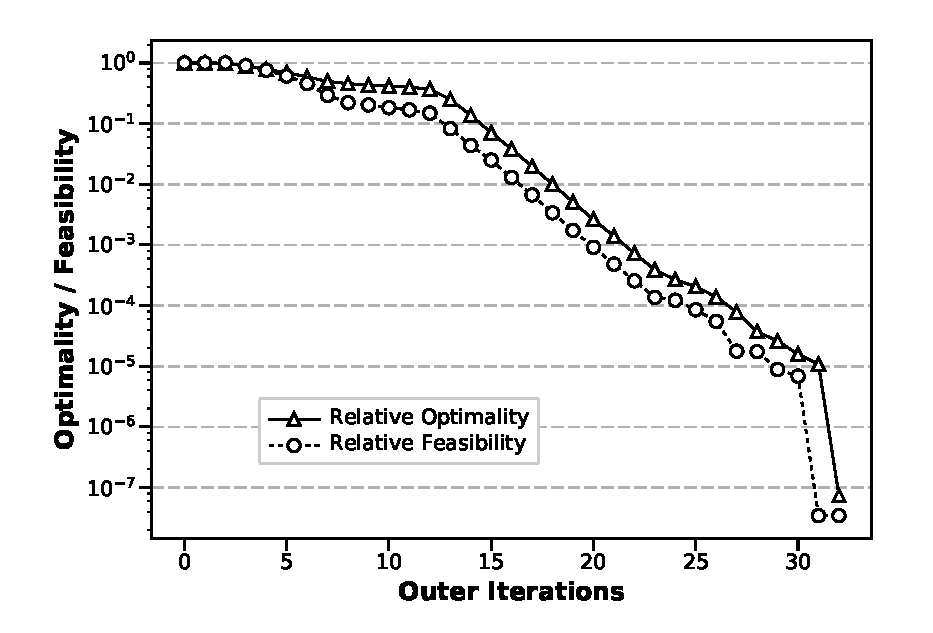
\includegraphics[clip,width=0.6\columnwidth]{./figs/nonconvex_100_1.eps}%
  \caption{Convergence Plot}
  \label{fig:nonconvex}
\end{figure}

The solutions from the optimization are checked against analytical true solutions, and all the stationery points in negative quadratic systems are successfully bypassed. Notice that for this test problem, the maximum nonconvexity is set at $-1$. When the maximum nonconvexity is higher, the optimization method may take more iterations to converge or have some difficulty. 

\subsection{Constructed Quadratic Problem}
Next the method is tested on a constructed quadratic problem with linear inequality constraints to validate the SVD based preconditioner. The objective Hessian and constraint Jacobian matrices are constructed with known singular value distributions. The problem is formulated as follows:
\begin{equation*}
\begin{aligned}
&\underset{x \in R^n} {\text{min}}  
& & \frac{1}{2}x^T Q x + g^T x \\
&\underset{b \in R^n} {\text{s.t.}}  & & Ax \geq b  \\
\end{aligned}
\end{equation*}
where: 
\begin{equation*}
\begin{aligned}
A &= U \Sigma V^\ast  \quad U \ \text{and} \ V \textrm{are randomly generated orthonormal matrix }, A \in \mathbb{R}^{n\times n} \\ 
\Sigma &= 10*diag(\sigma_1, ... \sigma_i, ... \sigma_k, \sigma_k, \sigma_k, ... ) \quad \textrm{with} \ \sigma_i = \frac{1}{i^2},\\
Q &= E\Lambda E^T  \quad  E \ \textrm{is a permutation of the Identity matrix, or orthonormal matrix} \\
\Lambda &= 10*diag(\lambda_1, ...\lambda_i, ...\lambda_t, \lambda_t, \lambda_t, ...) \quad \textrm{with} \ \lambda_i = \frac{1}{i}, 
\end{aligned}
\end{equation*}
The constant scalar $10$ in $\Sigma$ and $\Lambda$ is simply to increase the magnitude of the matrix $A$ and $Q$.  
Because $b$, $U$ and $V$ for the inequality constraints are all randomly generated, definitely some of the constraints are active. The random number generator seed is set to a certain value to make fair cross comparisons. 

In this problem, the constraint Jacobian and Hessian are constructed a-prior thus explicitly available. However, the optimization algorithm only use their matrix vector products. The previously mentioned SVD preconditioner is used. At the moment, $\sigma_i$ and $\lambda_i$ are all positive, making $Q$ positive definite. The value of $k$ and $t$ are randomly chosen to be a fixed positive value smaller than the number of design variables. This is to make the condition number of the matrix fixed, rather than hugely increasing with the dimension of the problem. 

Notice that this test problem does not have state vectors, and the total constraint Jacobian exists in explicit matrix form to be used by SNOPT. For such problems, the new method cannot track the linear solver cost exactly, and SNOPT tracks cost differently, using the number of objective and sensitivity function evaluations. Therefore, the CPU computing time is used as the x-axis. When running the tests, all other routines on the computer are closed to make a fair comparison as much as possible. 

A range of different number of design variables from $100$ to $500$ is tested, and the 
convergence plots for the $200$ and $500$ cases are selected and shown in Fig. \ref{fig:toy} below. The convergence for other cases have similar trends and is omitted here for saving space. In the legend, Eye optimality Eye feasibility refers to unpreconditioned case; SVD optimality and feasibility refers to the new method with the matrix-free preconditioner mentioned before; SNOPT optimality and feasibility are the convergence results from SNOPT. 

It can be seen that as the problem dimension increases, the matrix-based optimization method SNOPT takes longer time to complete each step, while the new matrix-free optimization method uses roughly the same time. The bottom right subfigure in Fig. \ref{fig:ndvcosttoy} shows the CPU computing time cost versus number of design. 

\begin{figure}[H]
\centering
\subfloat{%
  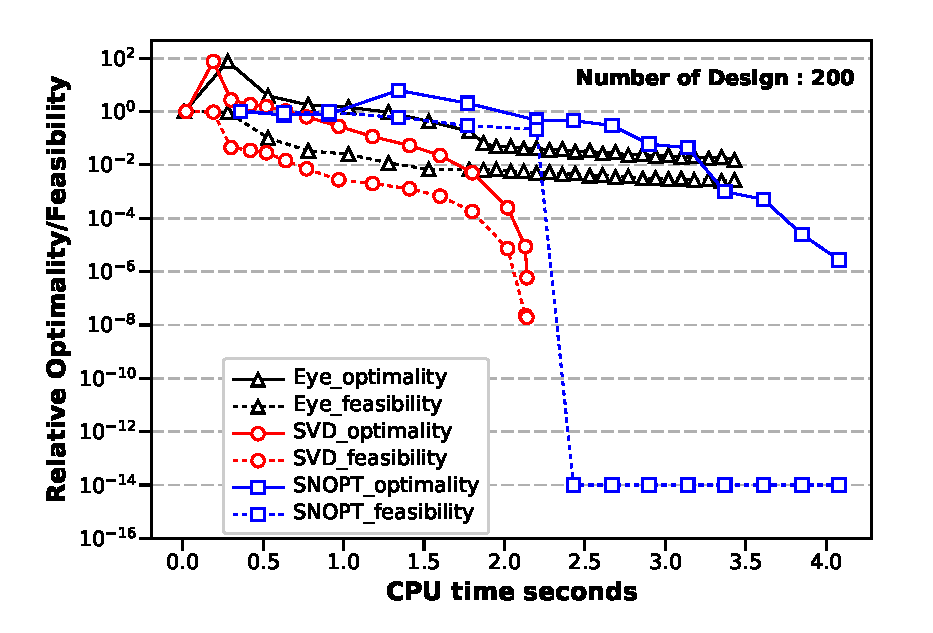
\includegraphics[clip,width=0.5\columnwidth]{./figs/200.eps}%
}
\subfloat{%
  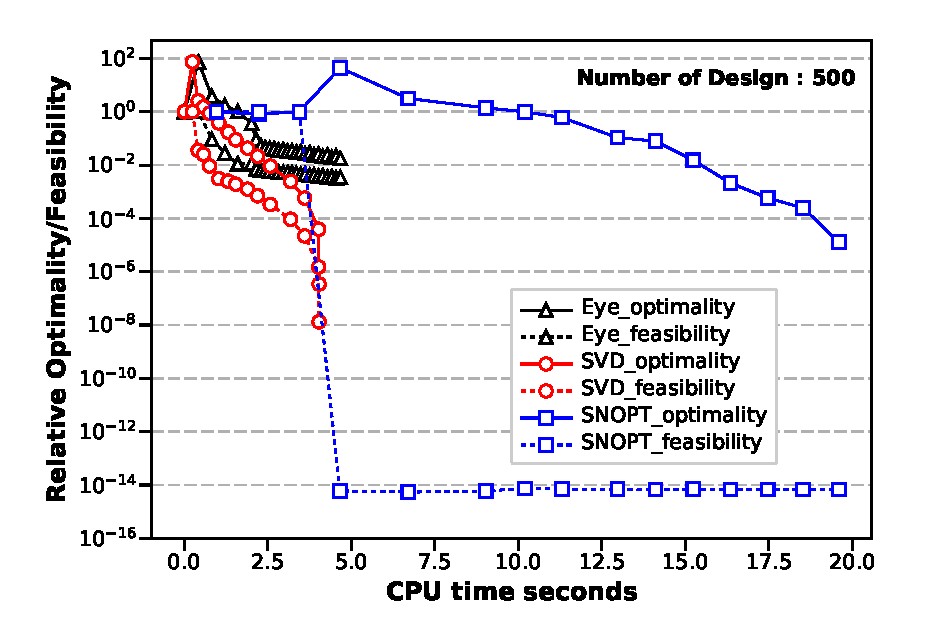
\includegraphics[clip,width=0.5\columnwidth]{./figs/500.eps}%5}

% \subfloat{%
%   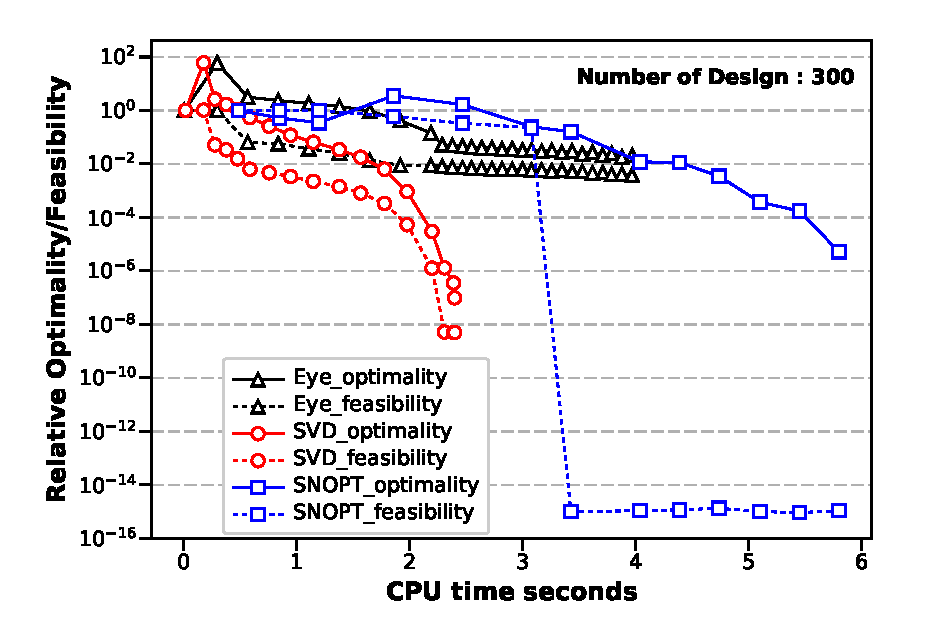
\includegraphics[clip,width=0.6\columnwidth]{./figs/300.eps}%
% }
% \subfloat{%
%   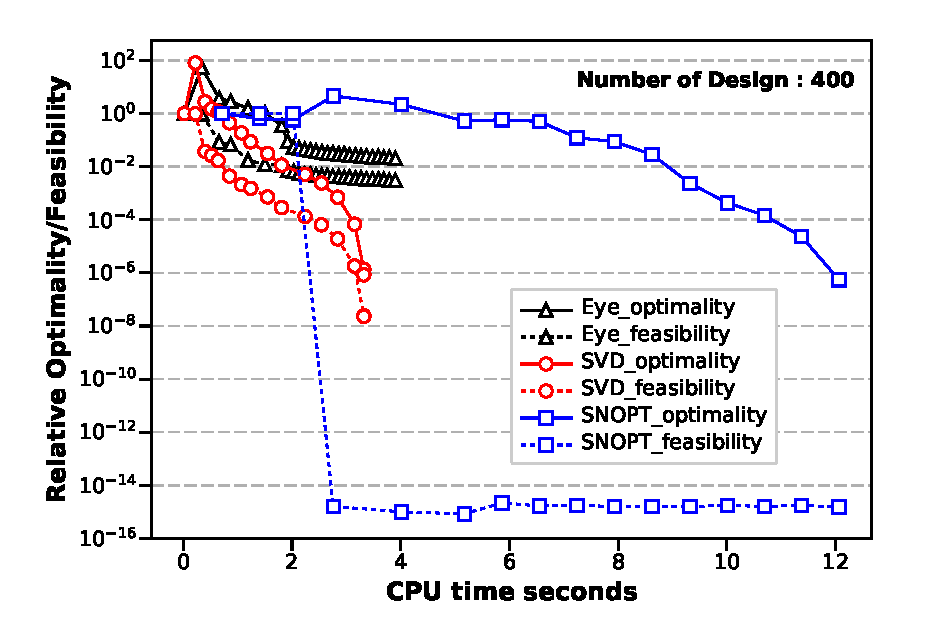
\includegraphics[clip,width=0.6\columnwidth]{./figs/400.eps}%
% }

% \subfloat{%
%   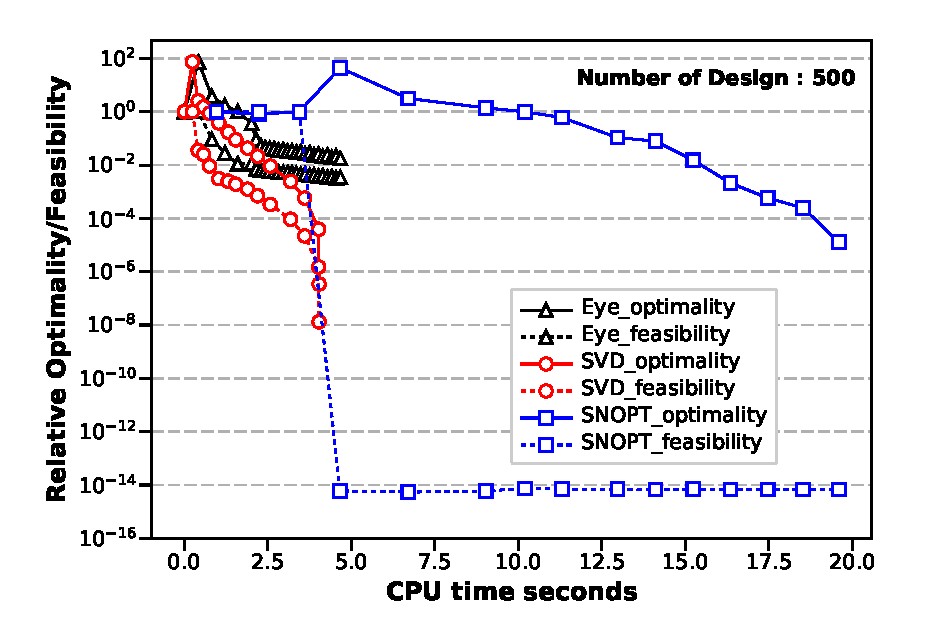
\includegraphics[clip,width=0.5\columnwidth]{./figs/500.eps}%
% }
}
\caption{Convergence Plots for increasing dimensions}
\label{fig:toy}
\end{figure}

\begin{figure}[H]
  \centering
  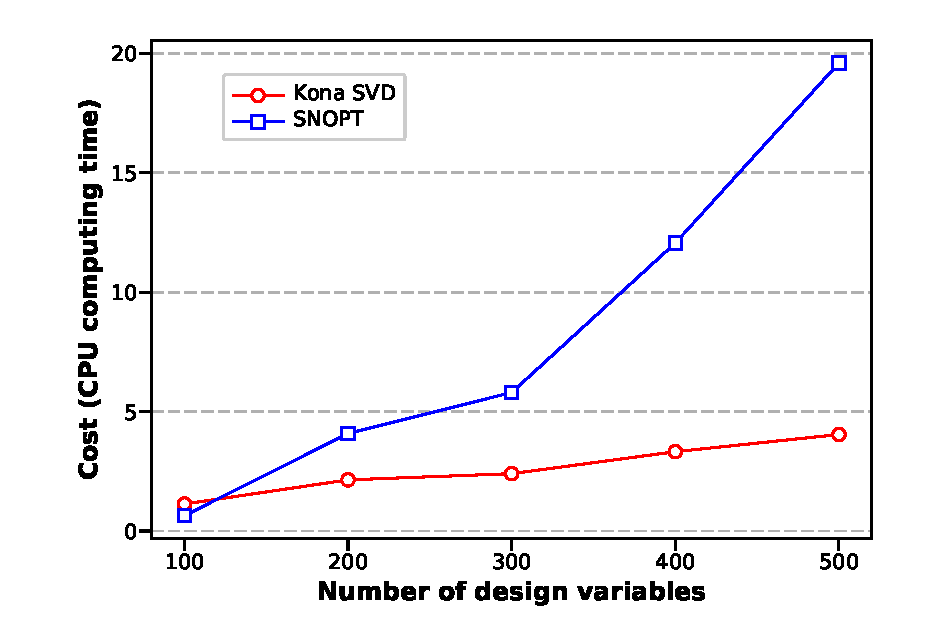
\includegraphics[clip,width=0.5\columnwidth]{./figs/ndv_cost.eps}%
  \caption{Scalability Performances}
  \label{fig:ndvcosttoy}
\end{figure}


\subsection{Stress-Constrained Mass Minimization}
The second test problem is a structural sizing design problem \cite{dener:scitech2016}. The design variables are plate thickness on a 2-D plate with one side fixed and the other side subject to an external force. Fig.\ref{fig:struct} illustrates the problem.
\begin{figure}[H]
  \centering
  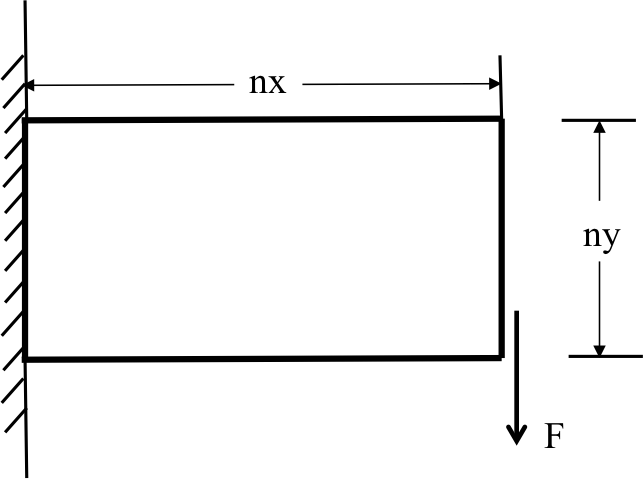
\includegraphics[width=0.5\textwidth]{./figs/structures.png}
  \caption{Plate thickness design problem}
  \label{fig:struct}
\end{figure}
where $nx$ and $ny$ are the number of elements along the horizontal and vertical direction. 

The objective function is the mass the of the plate, which directly depends on the thickness distribution, the design variables. The system is governed by the structural constitutive equations, with the displacements of each finite elements being the state variables. The stress distribution depends on the strain via Young's modulus, while the strain is related with the displacements. The constraints include lower and upper bound constraints on the design variables, and the von Mises stress constraint of the stress variables. The mathematical formulation is as follows:
\begin{equation*}
\begin{aligned}
\text{min}  \quad & \text{Mass}(x) &\\
\text{subject to} \quad & x_l \leq x \leq x_u  \\
 &  \sigma _{\textrm{Von Mises}} \leq  \sigma_{\text{allowed}} \\
\text{governed by} \quad &  \mathcal{F}(x, u) = 0 \\
\end{aligned}
\end{equation*}

The problem can be easily scaled up by increasing $nx$ and $ny$. We use small, medium, large to represent different scale of the problem:
\begin{center}
\begin{tabular}{ c c c c }
Case & nx  & ny & Number of design \\
\hline
 Small &   16 & 8 & 128 \\ 
 Medium &  32 & 16 & 512 \\  
 Large & 64 & 32 & 2048   
\end{tabular}
\end{center}

As the number of design increases, the number of singular values in the SVD approximation has to increase accordingly in order to capture sufficient features of the matrix \eqref{eq:lansvd2}. When the number of design variables is fixed, using more singular values can increase the convergence rate of the Krylov method more effectively, as shown in Fig. \ref{fig:svdrank} below. For this problem, when the number of design variables increases, more singular values need to be used to maintain the effectiveness of the preconditioner.   
\begin{figure}[H]
  \centering
  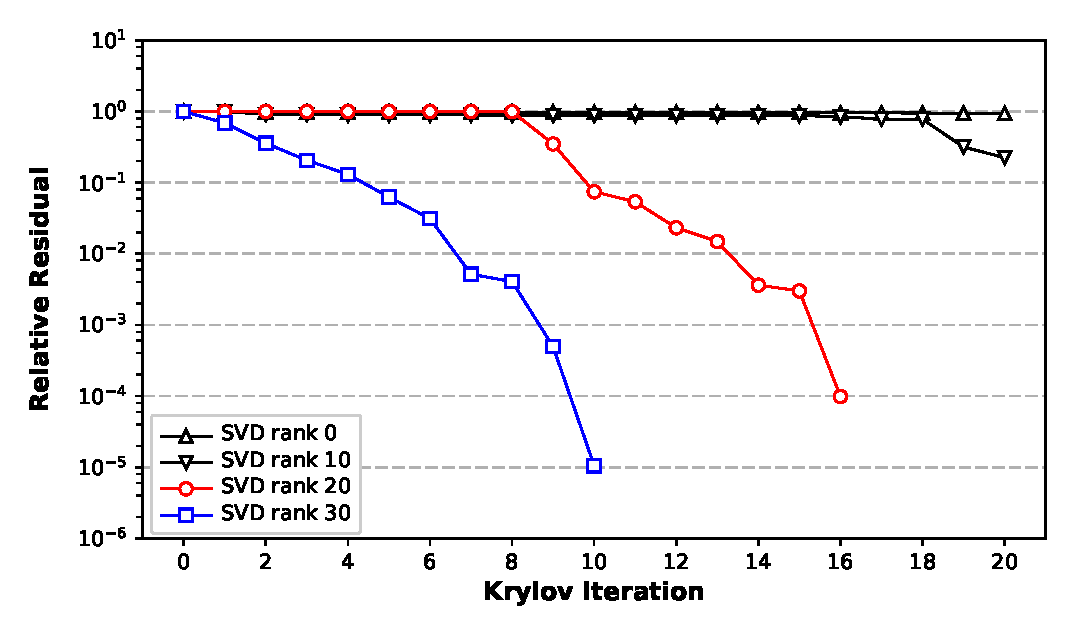
\includegraphics[width=0.6\textwidth]{./figs/svd_rank.eps}
  \caption{SVD rank on Krylov convergence rate}
  \label{fig:svdrank}
\end{figure}

Fig. \ref{fig:struct2} below shows the convergence plots on the small, medium and large problem. Each plot contains the optimality and feasibility iteration using the Homotopy method with Identity preconditioner, matrix-free preconditioner, and SNOPT.  When using the Identity preconditioner, it is very difficult for the iterative Krylov solver to make progress, as the KKT system is very ill-conditioned when $\mu$ gets close to zero. For the matrix-free preconditioner, the increasing cost with scaling dimension are mainly driven by the increasing number of singular values. 

The y-axis in Fig. \ref{fig:struct2} shows the change of relative optimality and absolute feasibility with cost. As can be seen, using the Homotopy optimization method with the matrix-free preconditioner can effectively bring the optimality and feasibility down to satisfactory tolerances. SNOPT takes longer time to converge, as it spends more resources on computing and storing the total constraint Jacobians. For the large scale problem, SNOPT struggles to converge. We suspect the constraint Jacobian might be rank-deficient for the large case. 
\begin{figure}[H]
\centering
% \subfloat{%
%   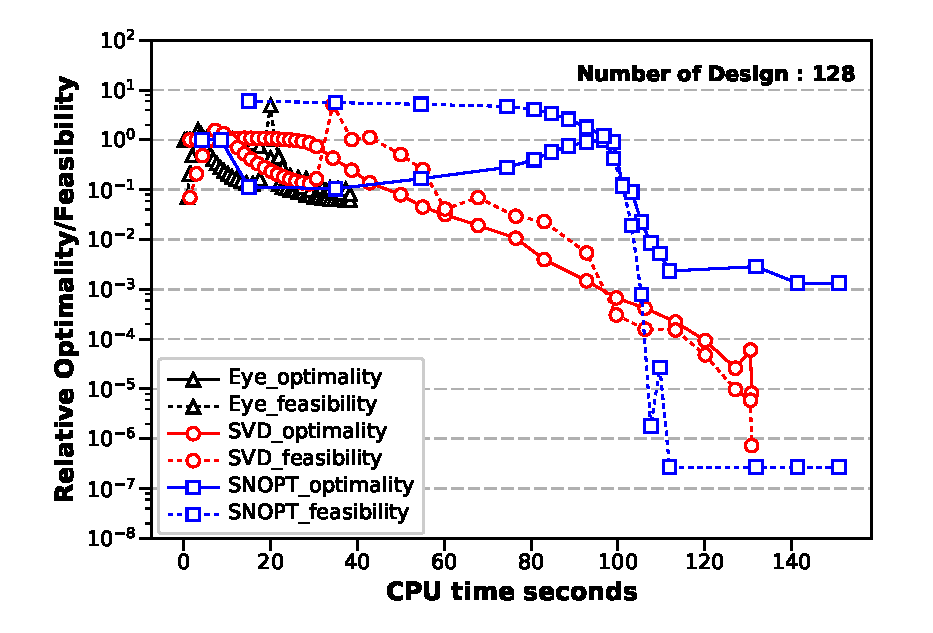
\includegraphics[clip,width=0.5\columnwidth]{./figs/tiny_time.eps}%
% }
\subfloat{%
  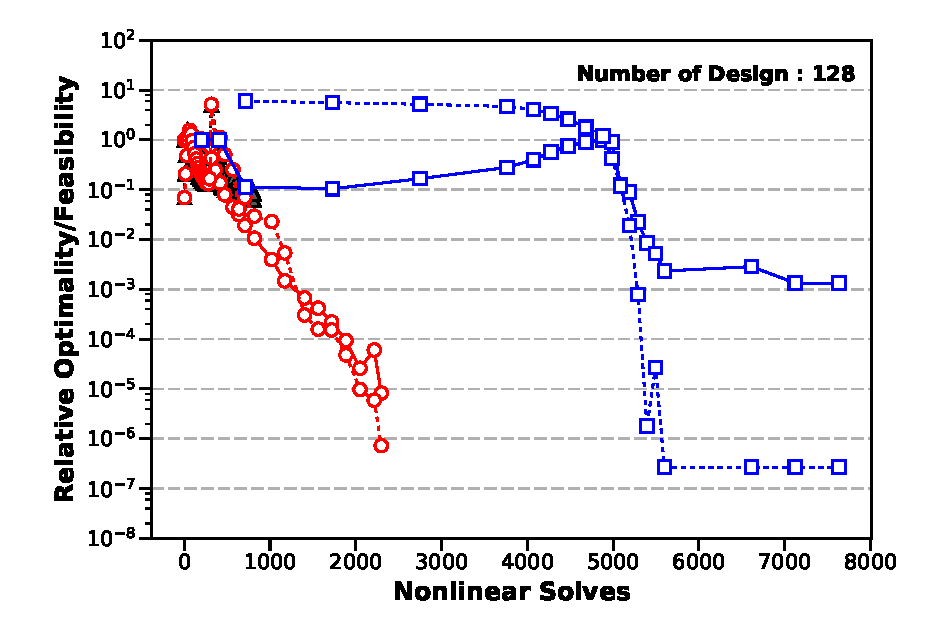
\includegraphics[clip,width=0.5\columnwidth]{./figs/tiny_cost.eps}%
}
\subfloat{%
  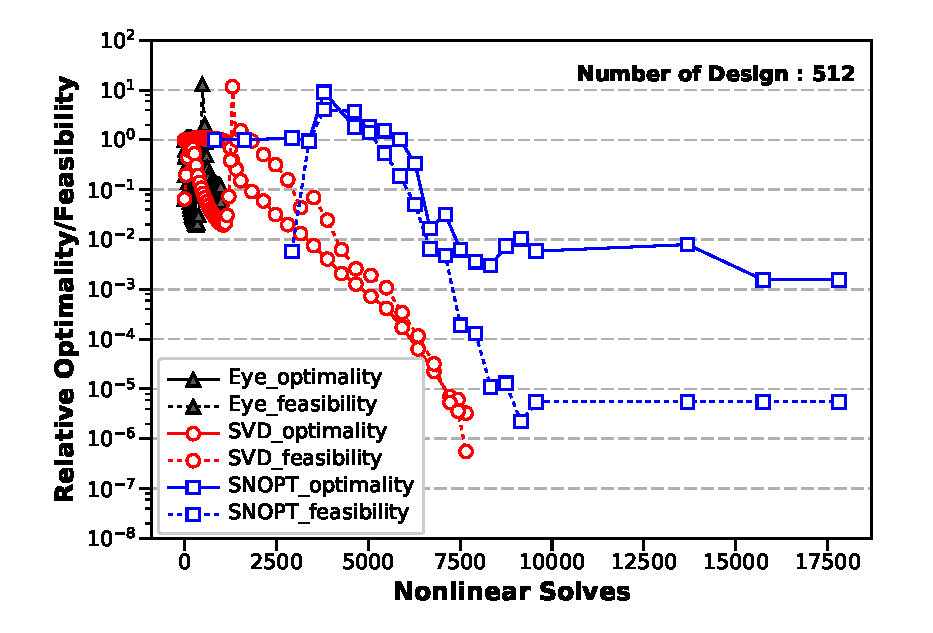
\includegraphics[clip,width=0.5\columnwidth]{./figs/small2_cost.eps}%
}

\subfloat{%
  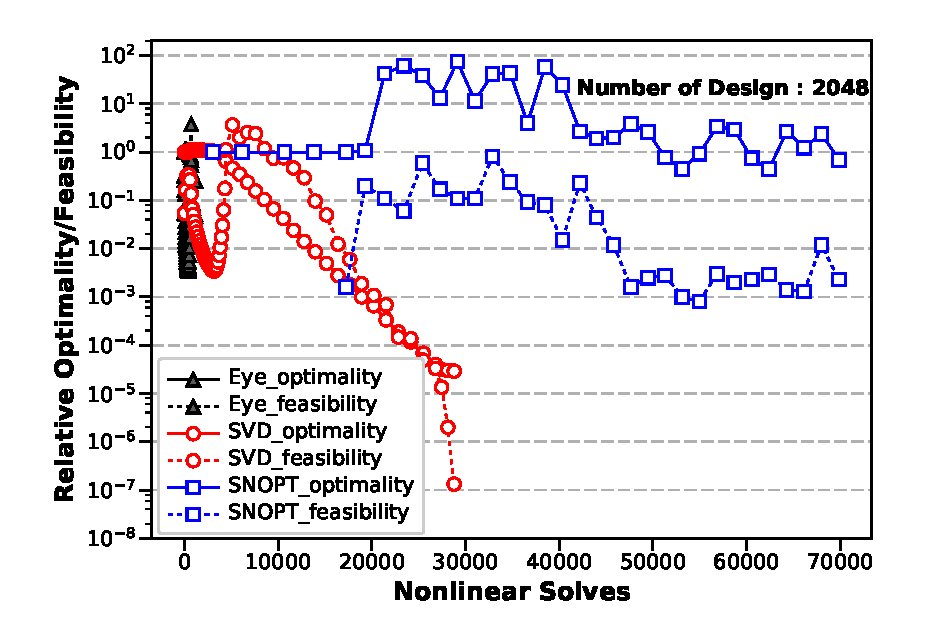
\includegraphics[clip,width=0.5\columnwidth]{./figs/medium2_cost.eps}%
}

% \subfloat{%
%   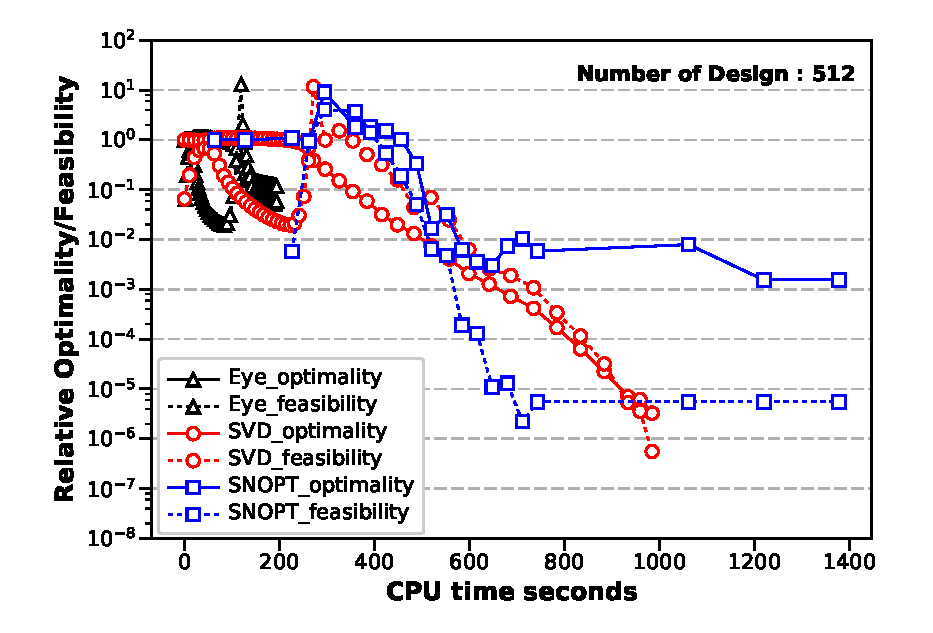
\includegraphics[clip,width=0.5\columnwidth]{./figs/small2_time.eps}%
% }
% \subfloat{%
%   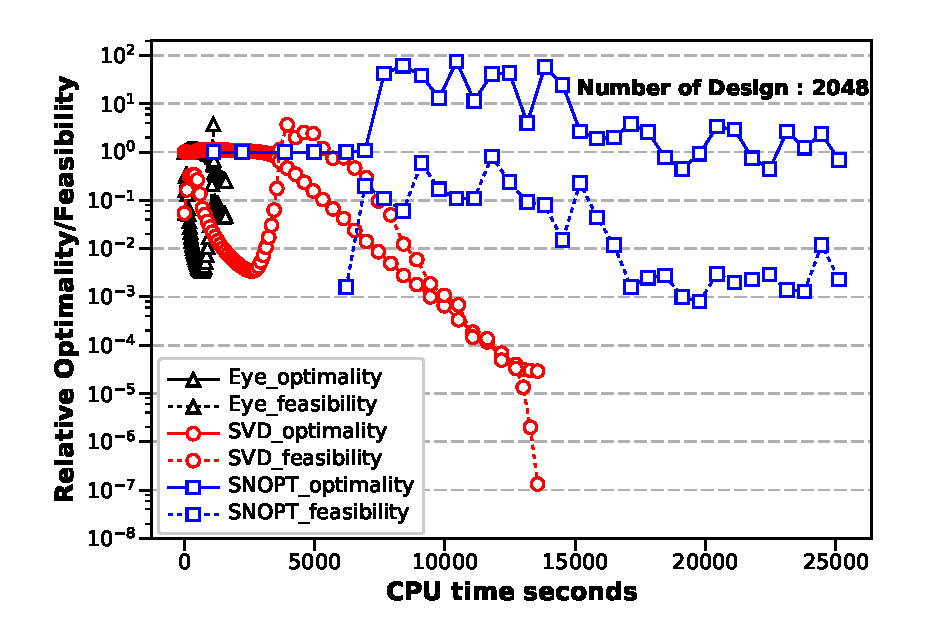
\includegraphics[clip,width=0.5\columnwidth]{./figs/medium2_time.eps}%
% }
\caption{Convergence Plots for Structural Problem}
\label{fig:struct2}
\end{figure}

The following Fig. \ref{fig:thick} shows the final optimal thickness distribution for the large case obtained by the new optimization method. The presented results agree with physical intuition for the problem. The blue color at one end of the spectrum means thinner thickness, while the brighter colors like yellow and red means thicker thickness.   

\begin{figure}[H]
\centering
%\subfloat[Small]{%
%  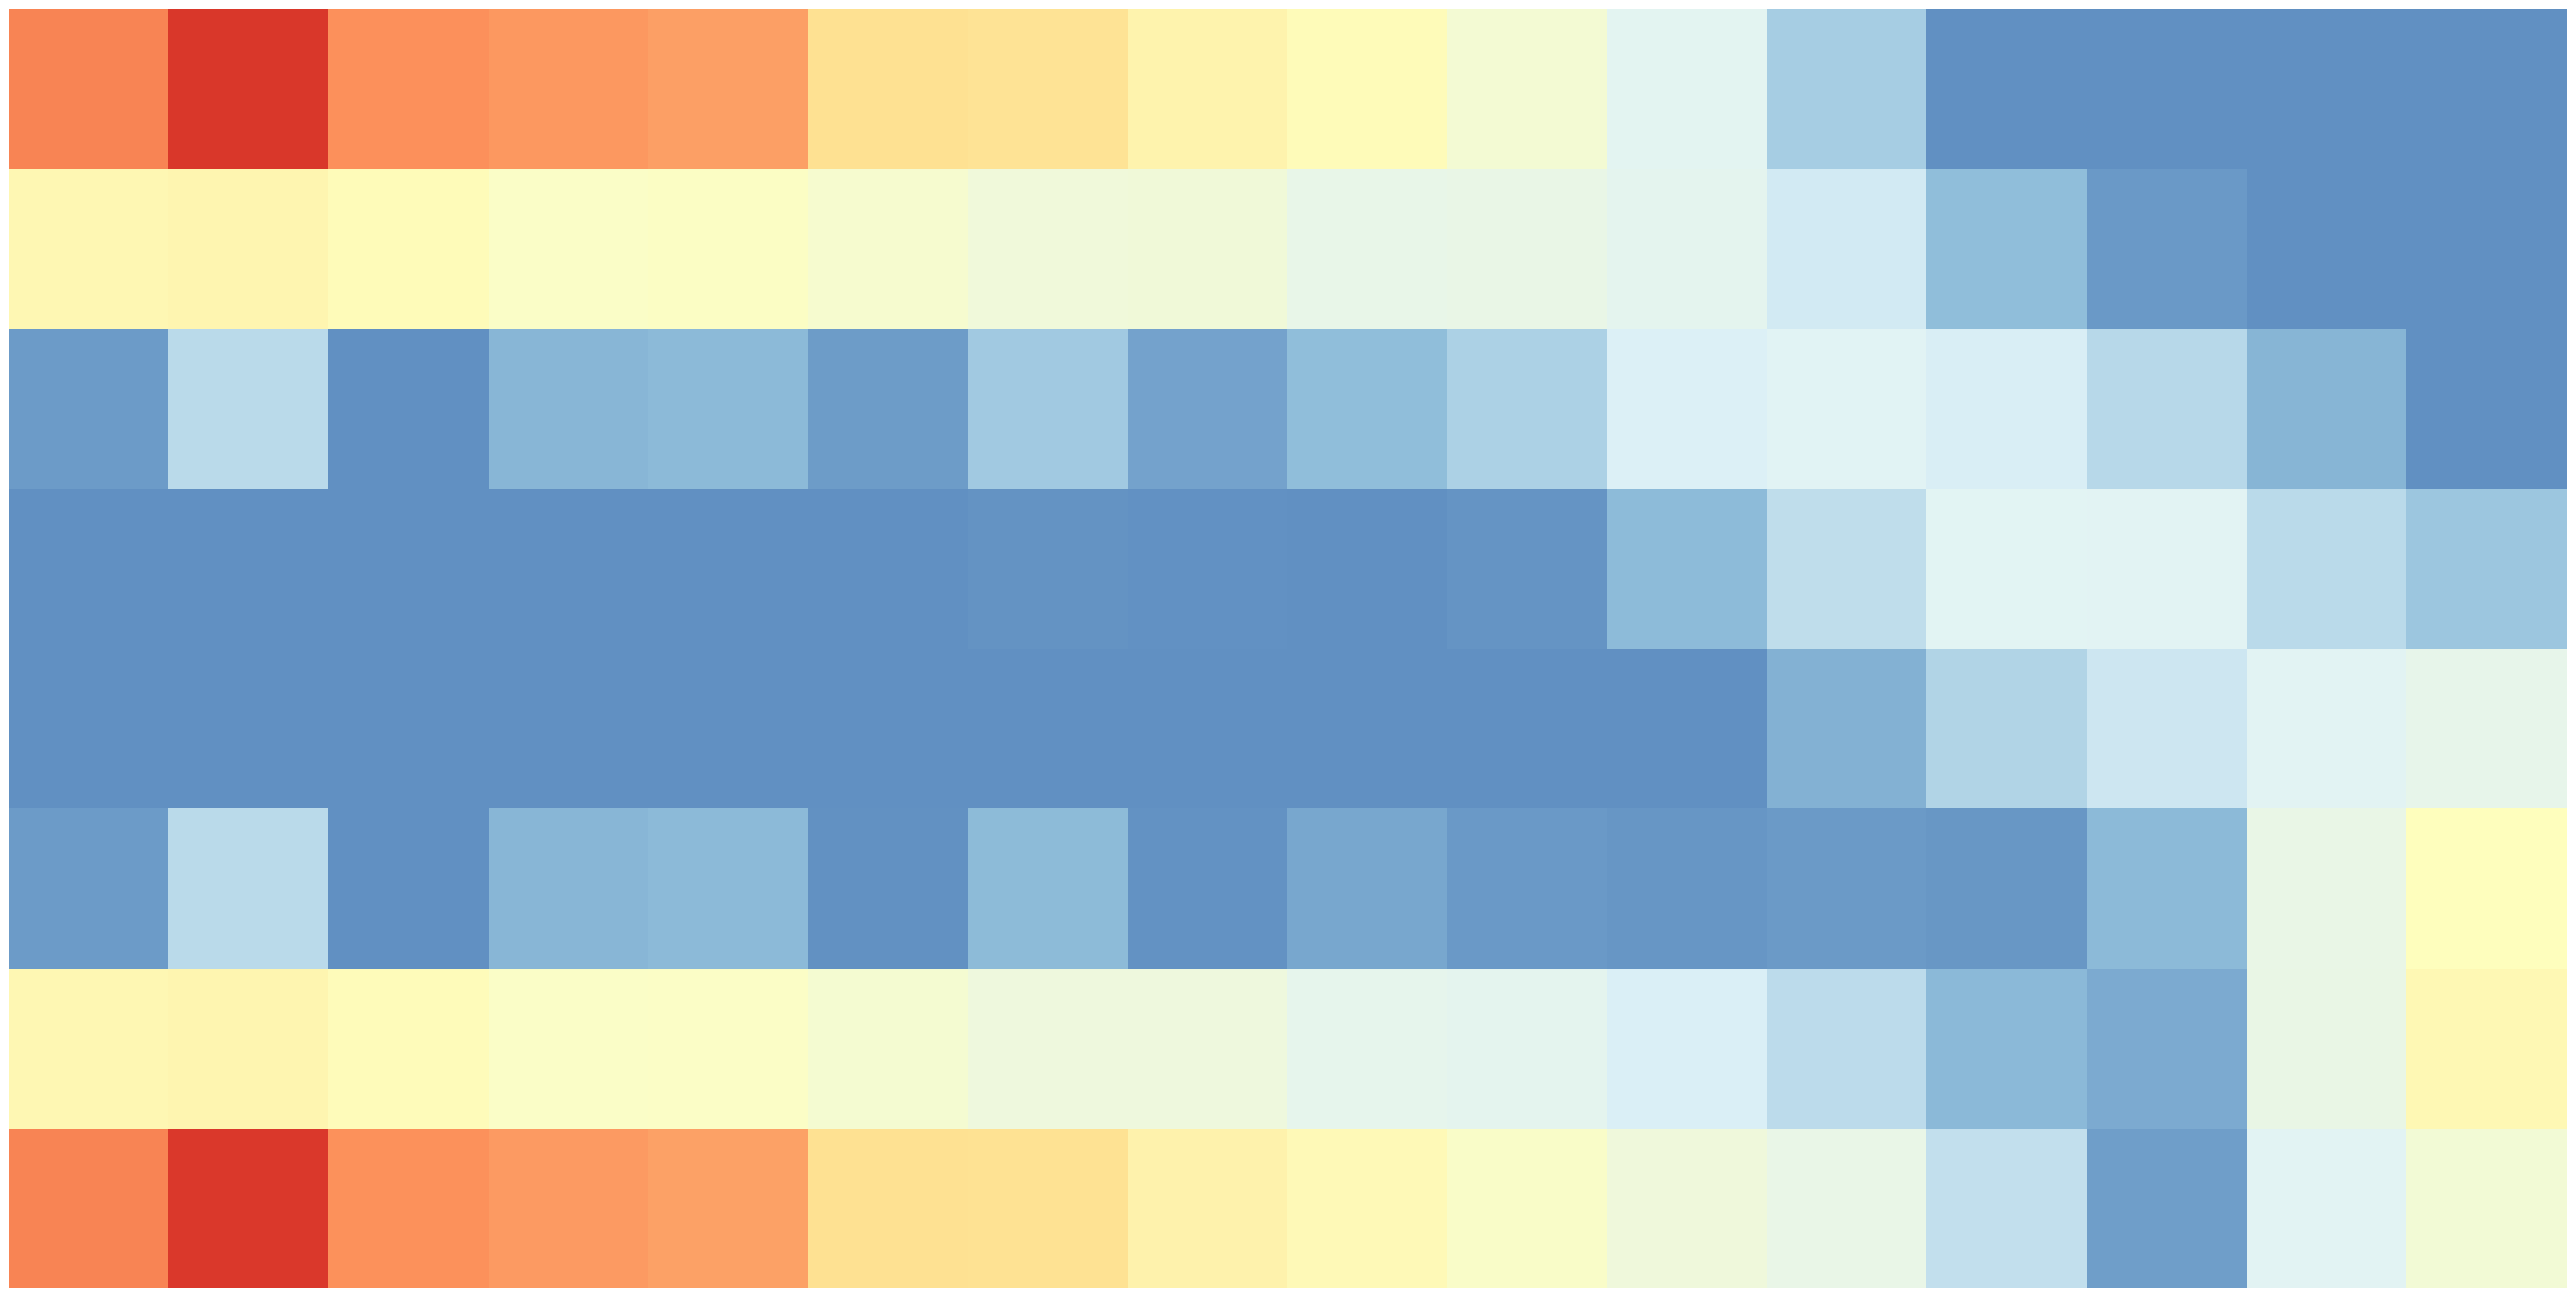
\includegraphics[clip,width=0.5\columnwidth]{./figs/kona_tiny.pdf}%
%}
%\subfloat[Medium]{%
%  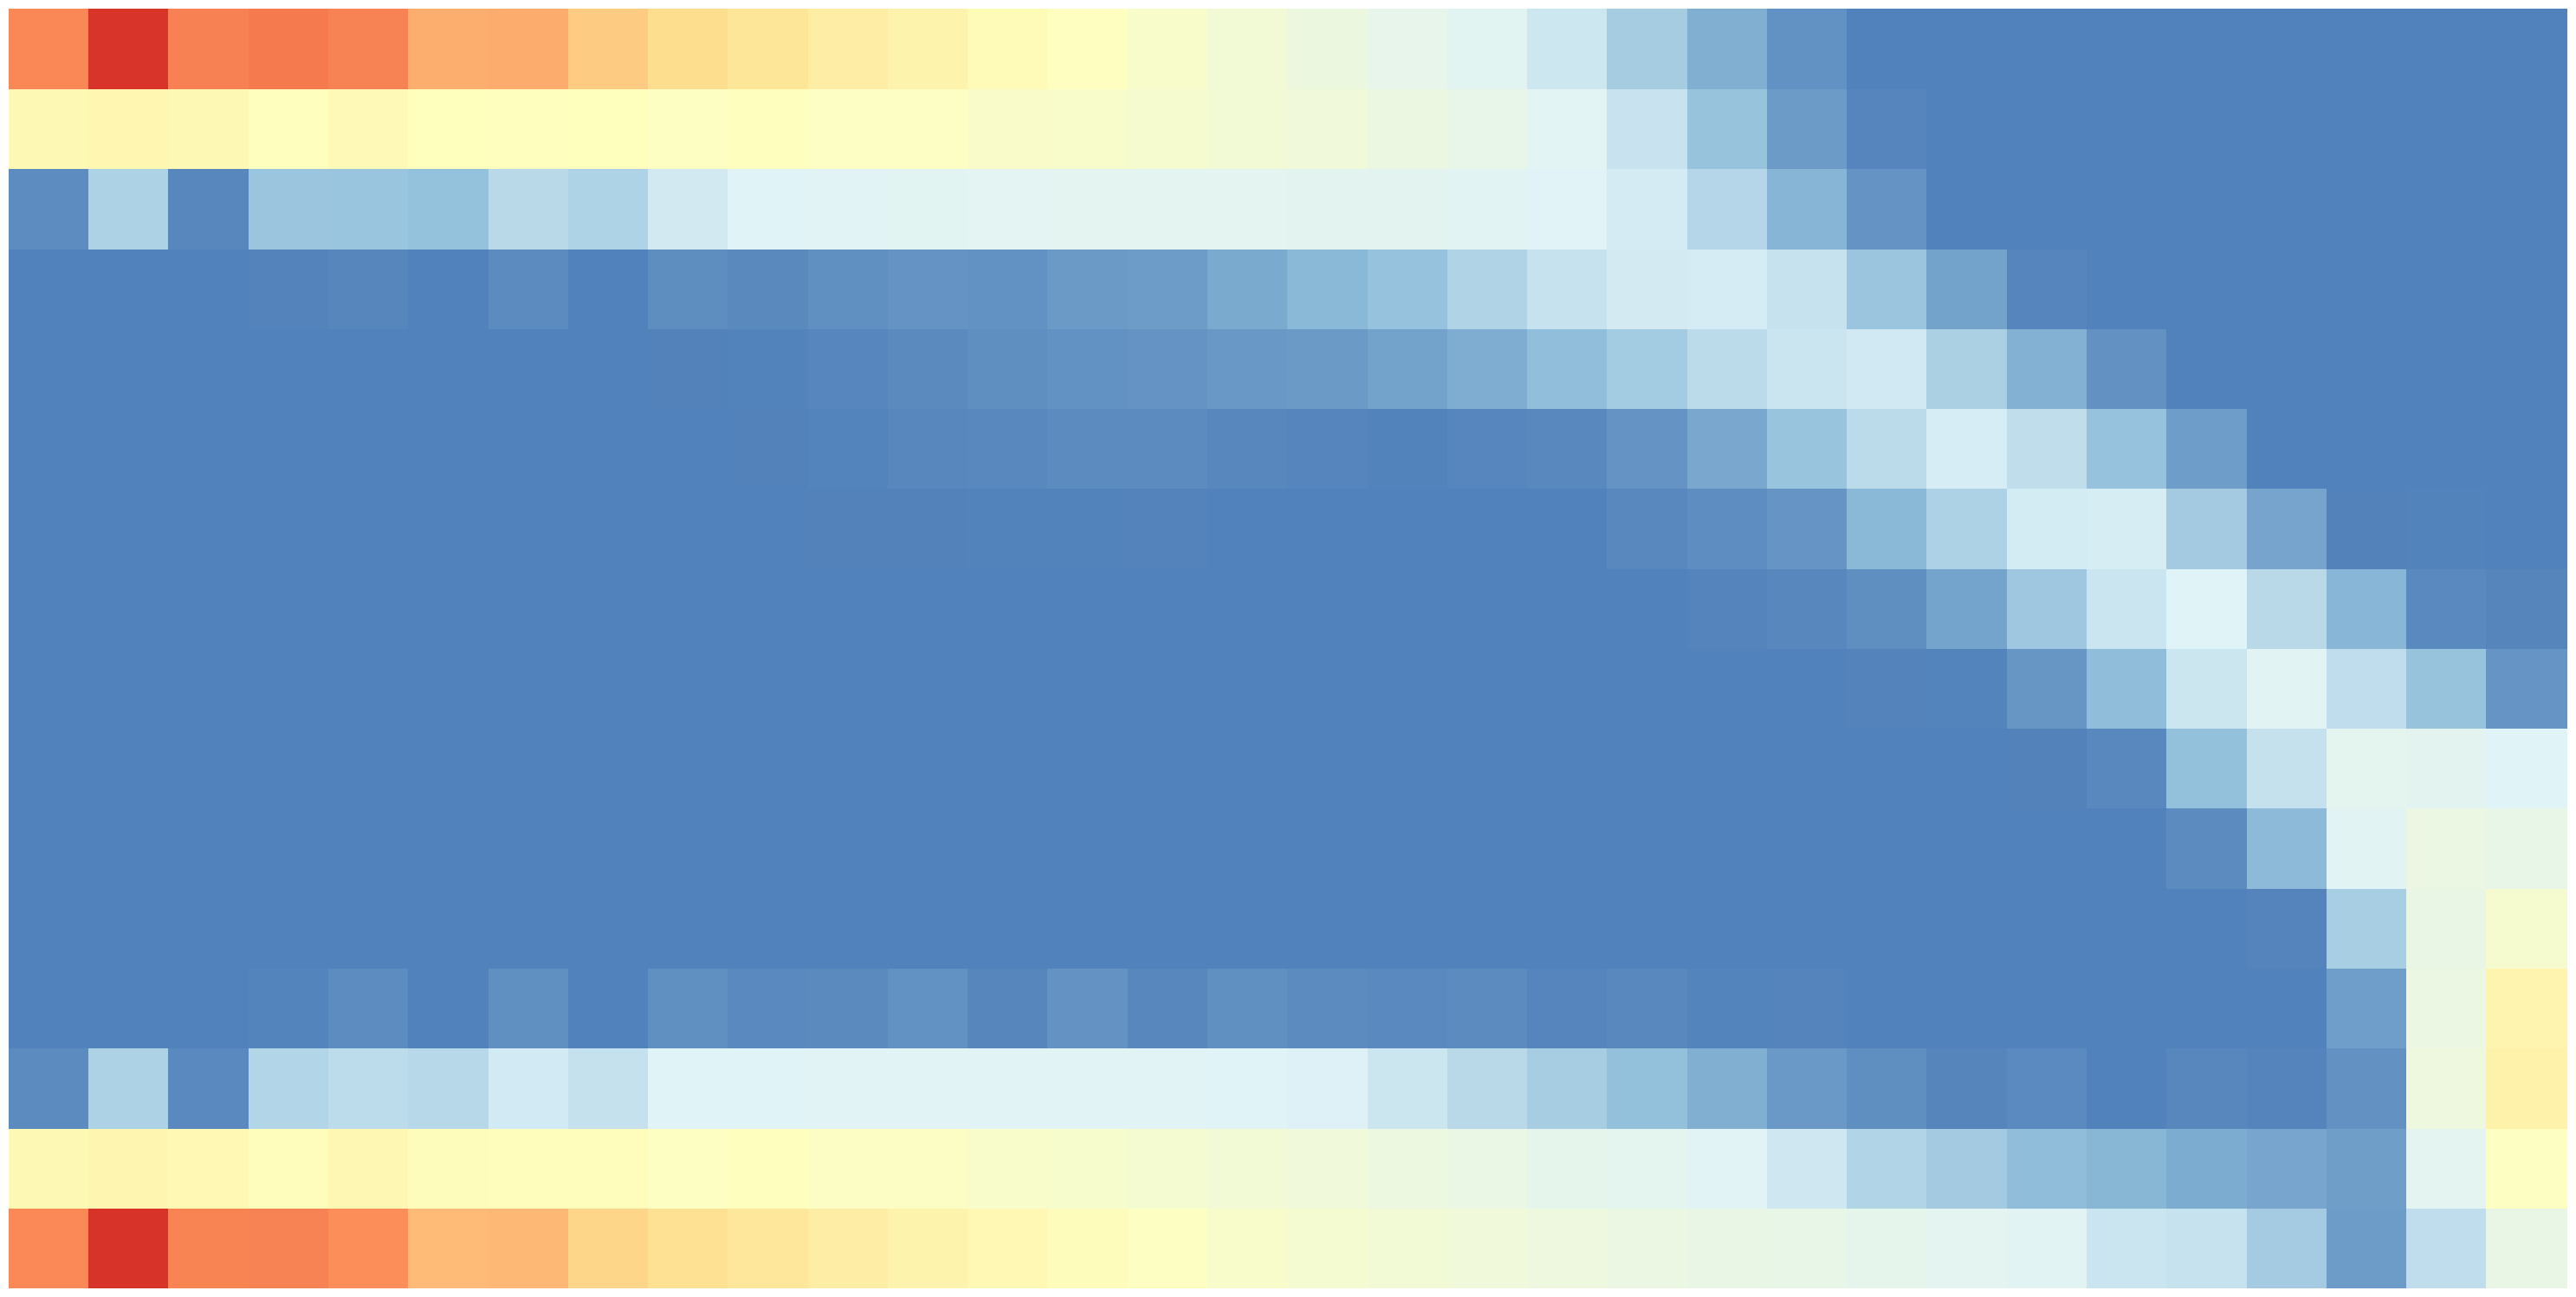
\includegraphics[clip,width=0.5\columnwidth]{./figs/small2_thick.pdf}%
%}


% \subfloat[Tiny: SNOPT thickness]{%
%   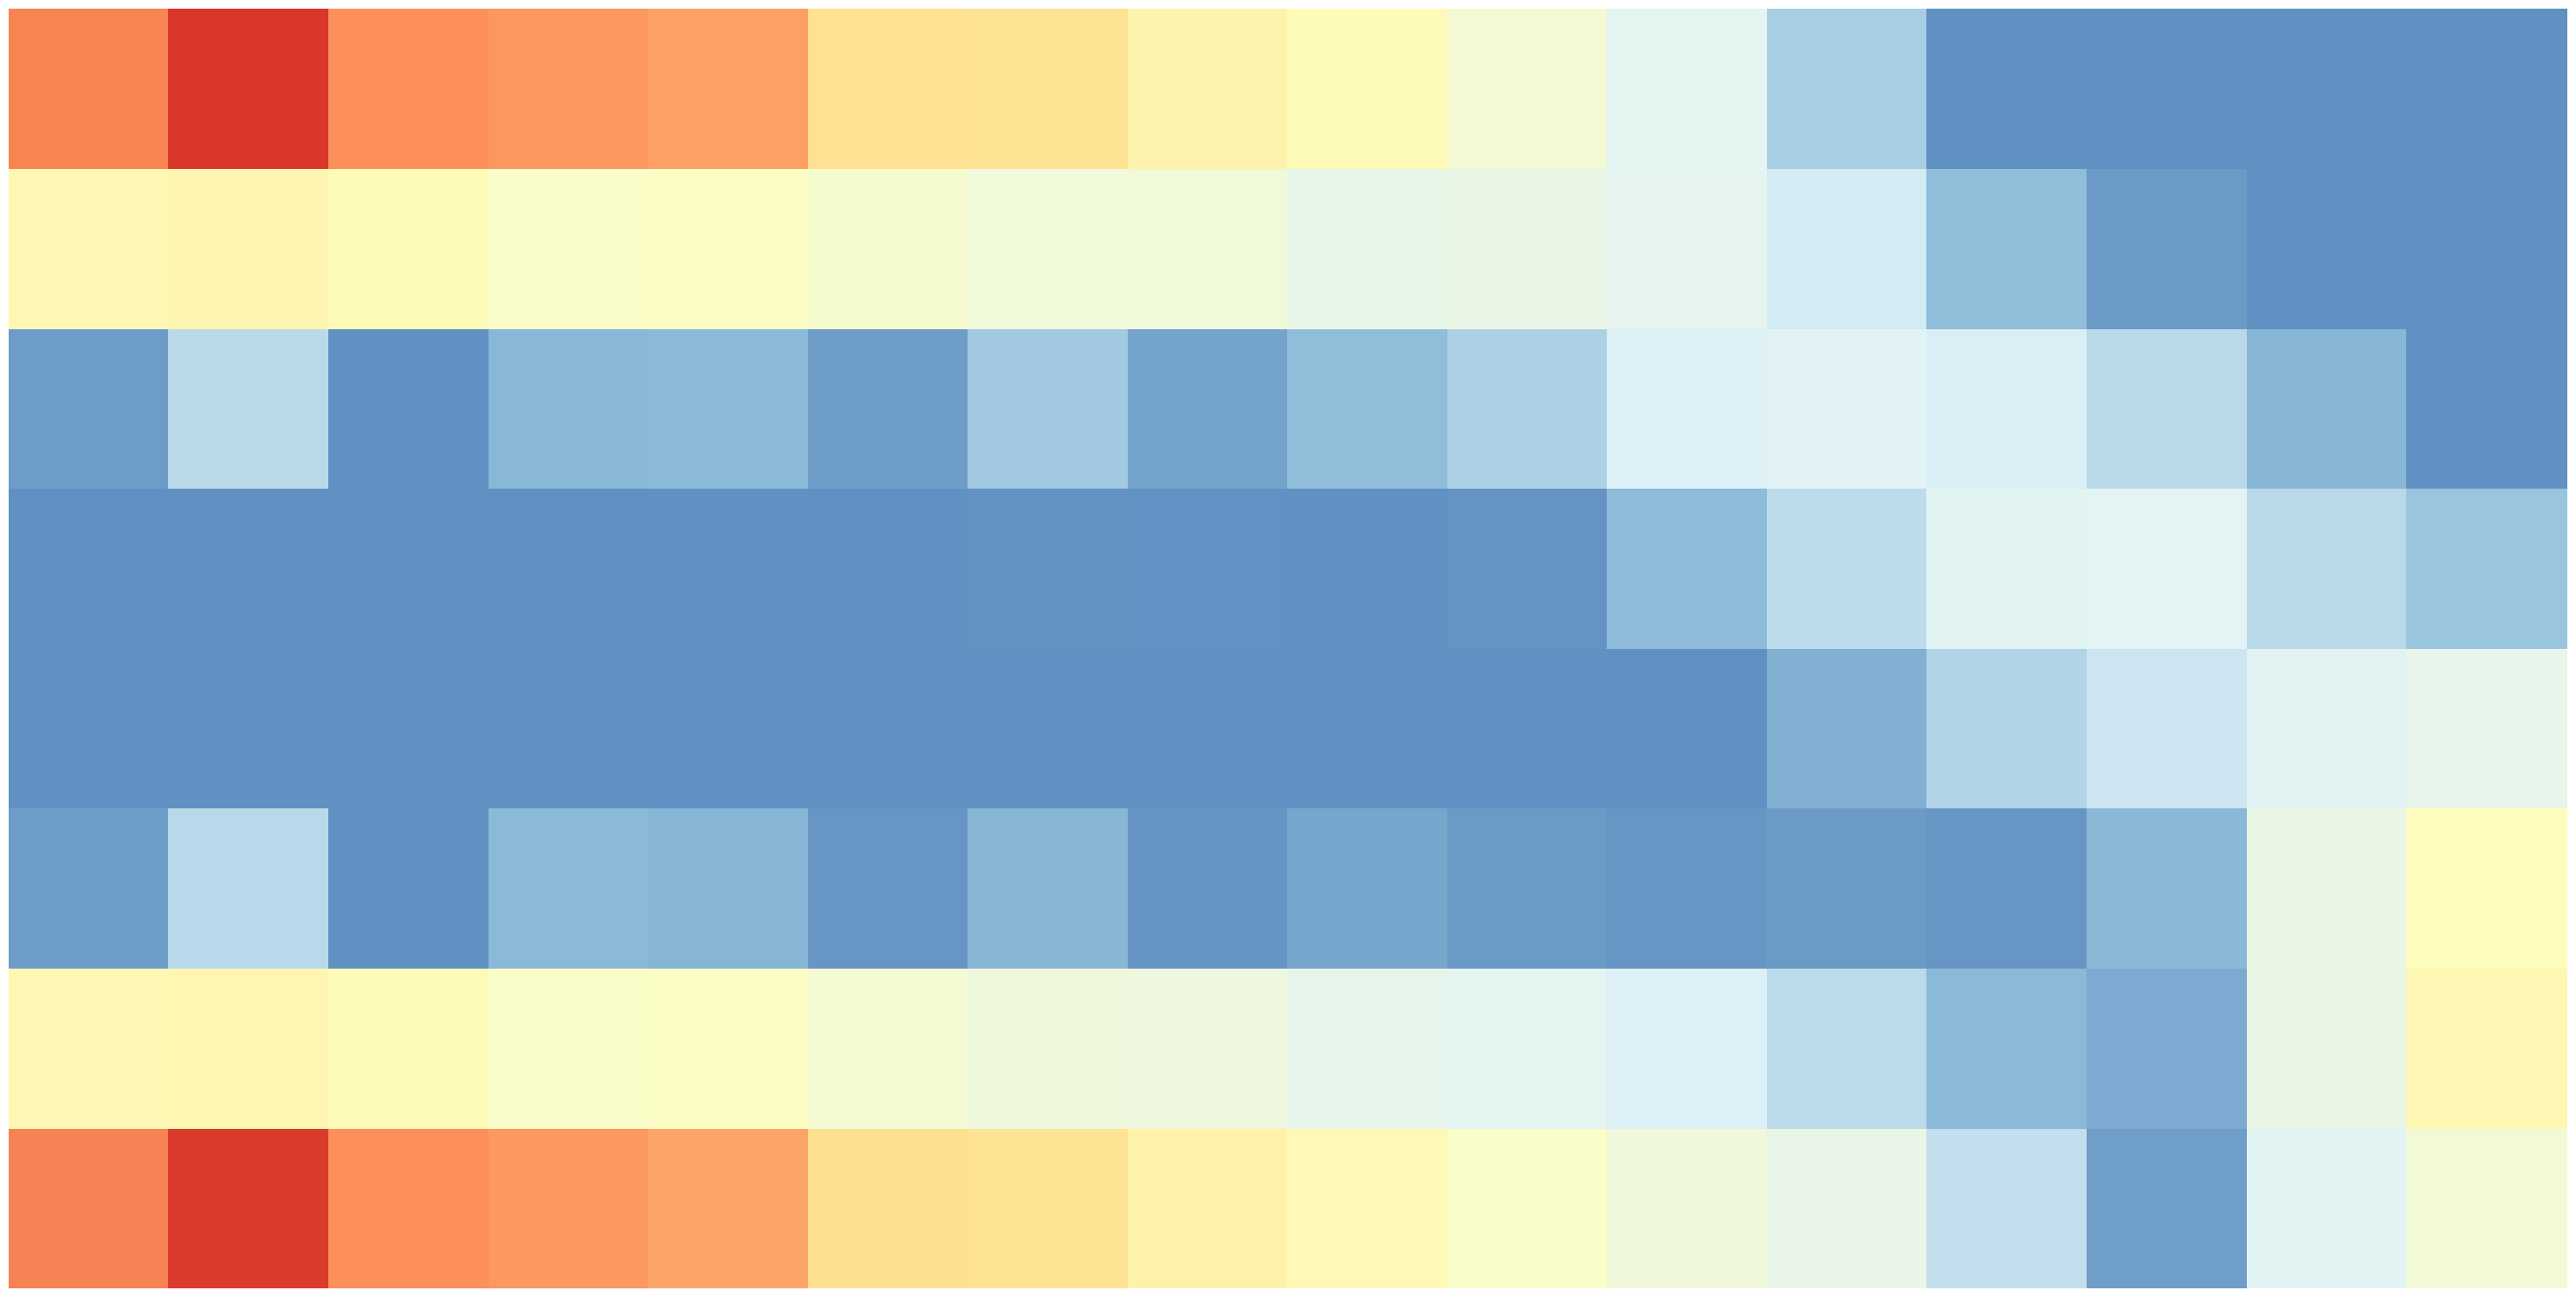
\includegraphics[clip,width=0.5\columnwidth]{./figs/snopt_tiny.pdf}%
% }

% \subfloat[Small: Kona thickness]{%
%   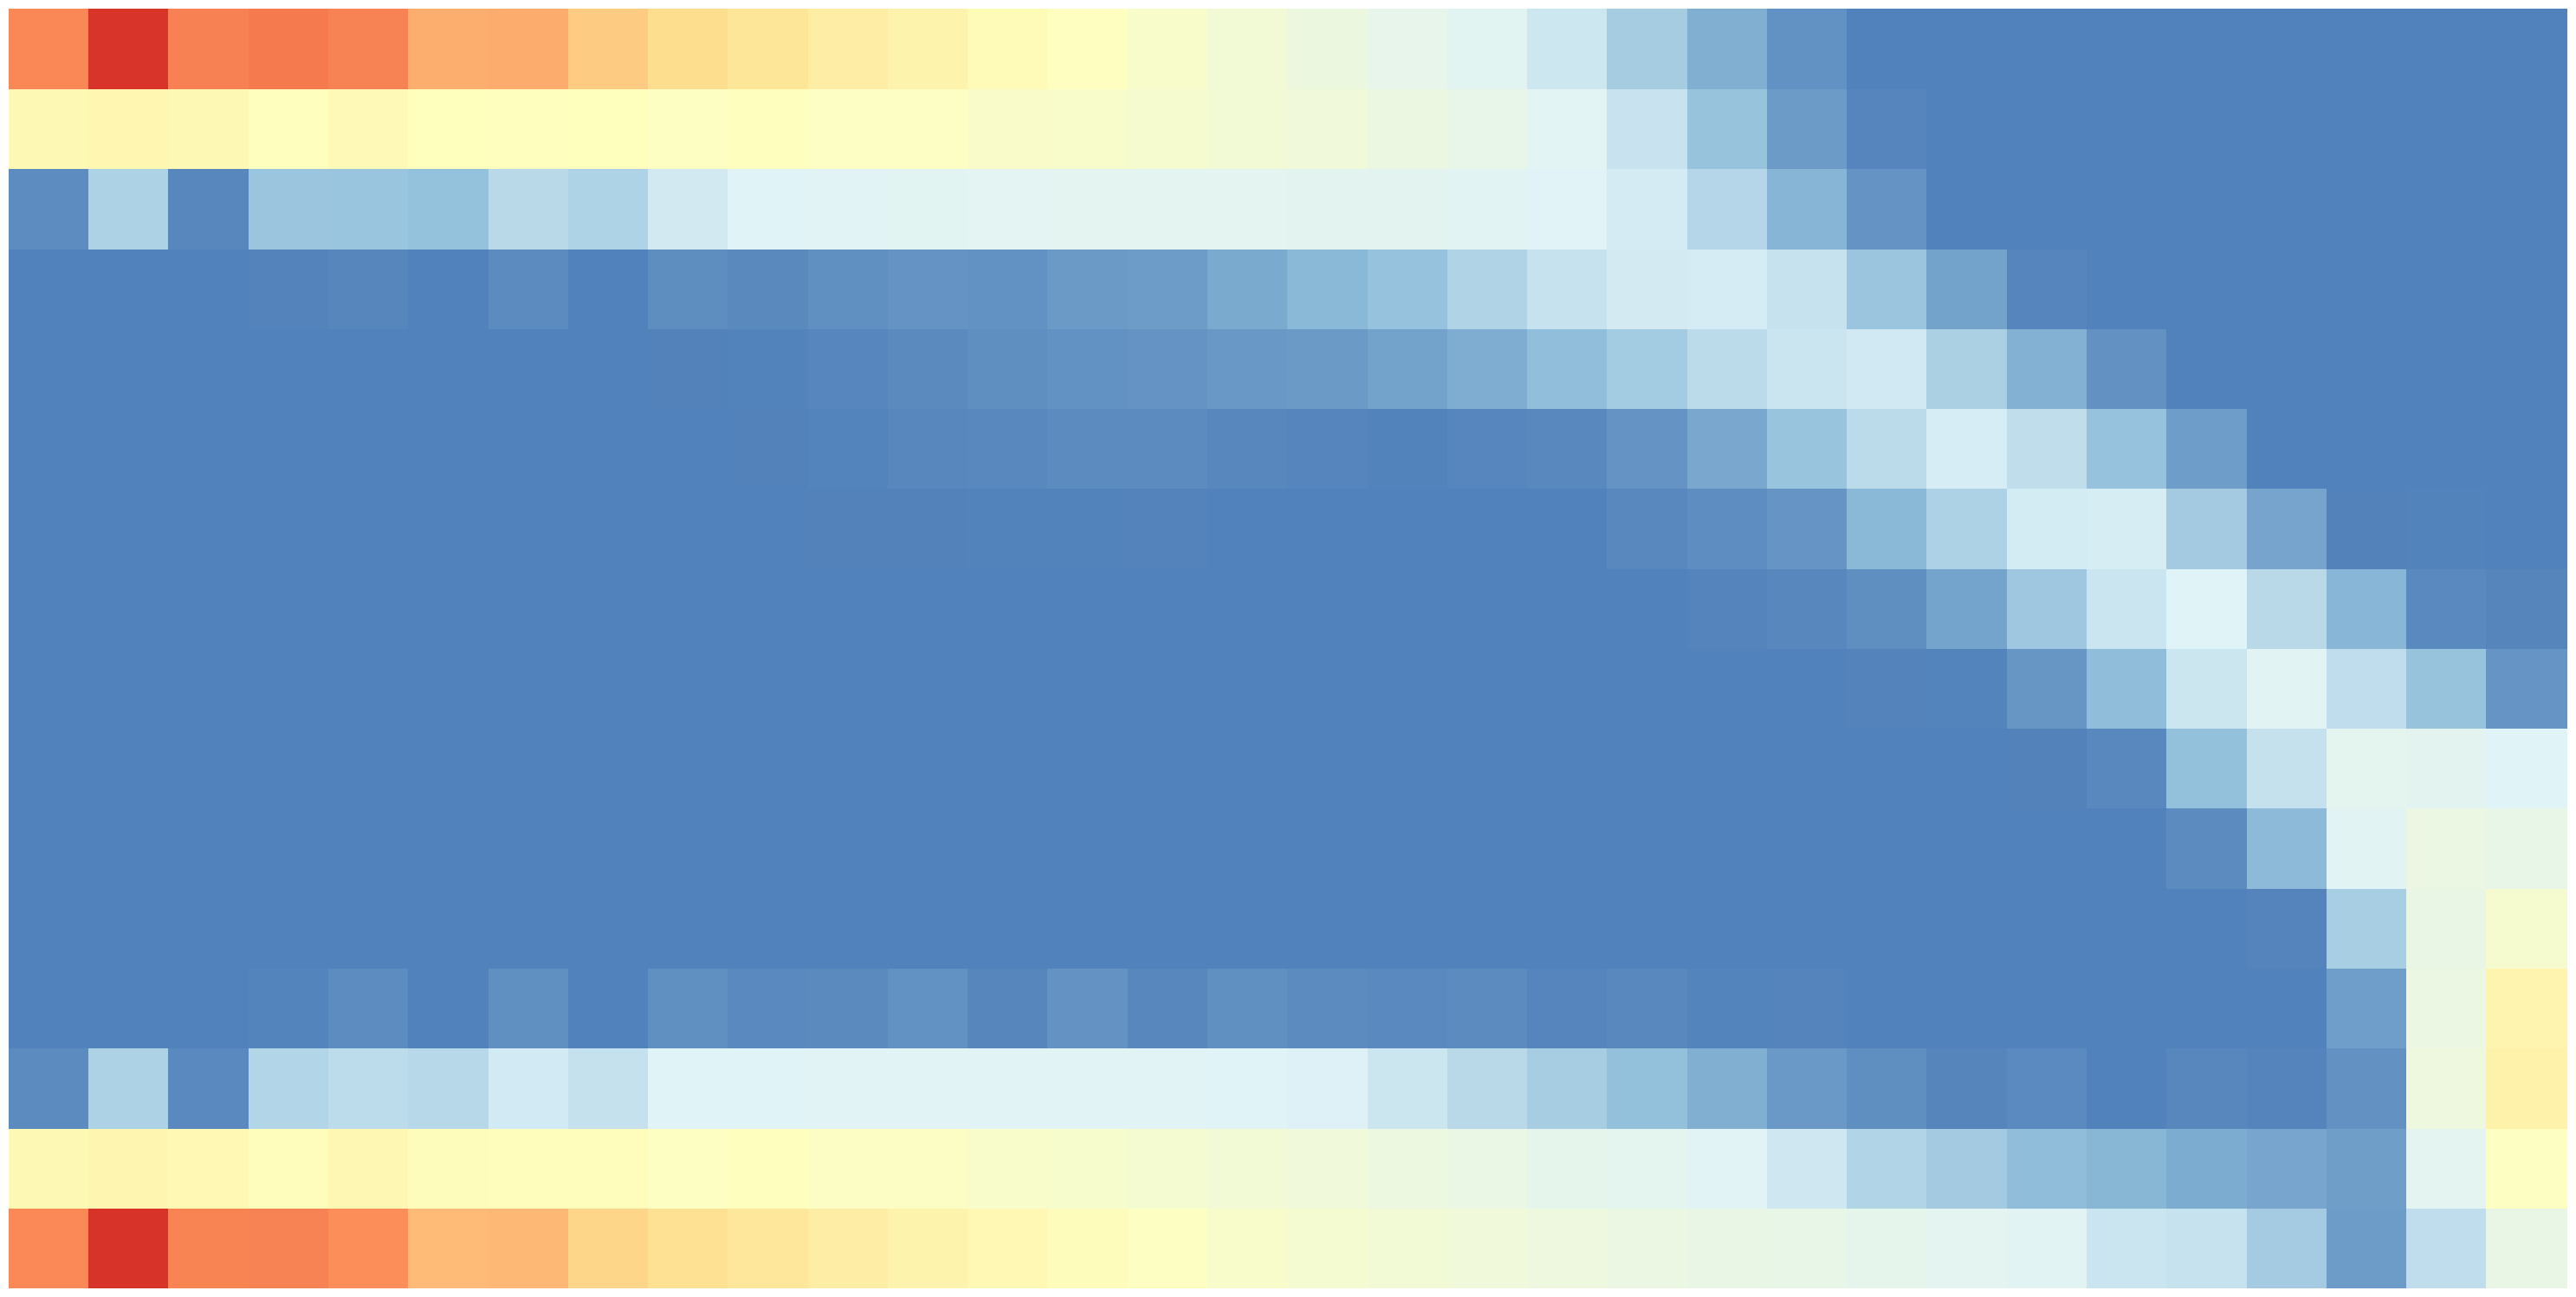
\includegraphics[clip,width=0.5\columnwidth]{./figs/small2_thick.pdf}%
% }
% \subfloat[Small: SNOPT thickness]{%
%   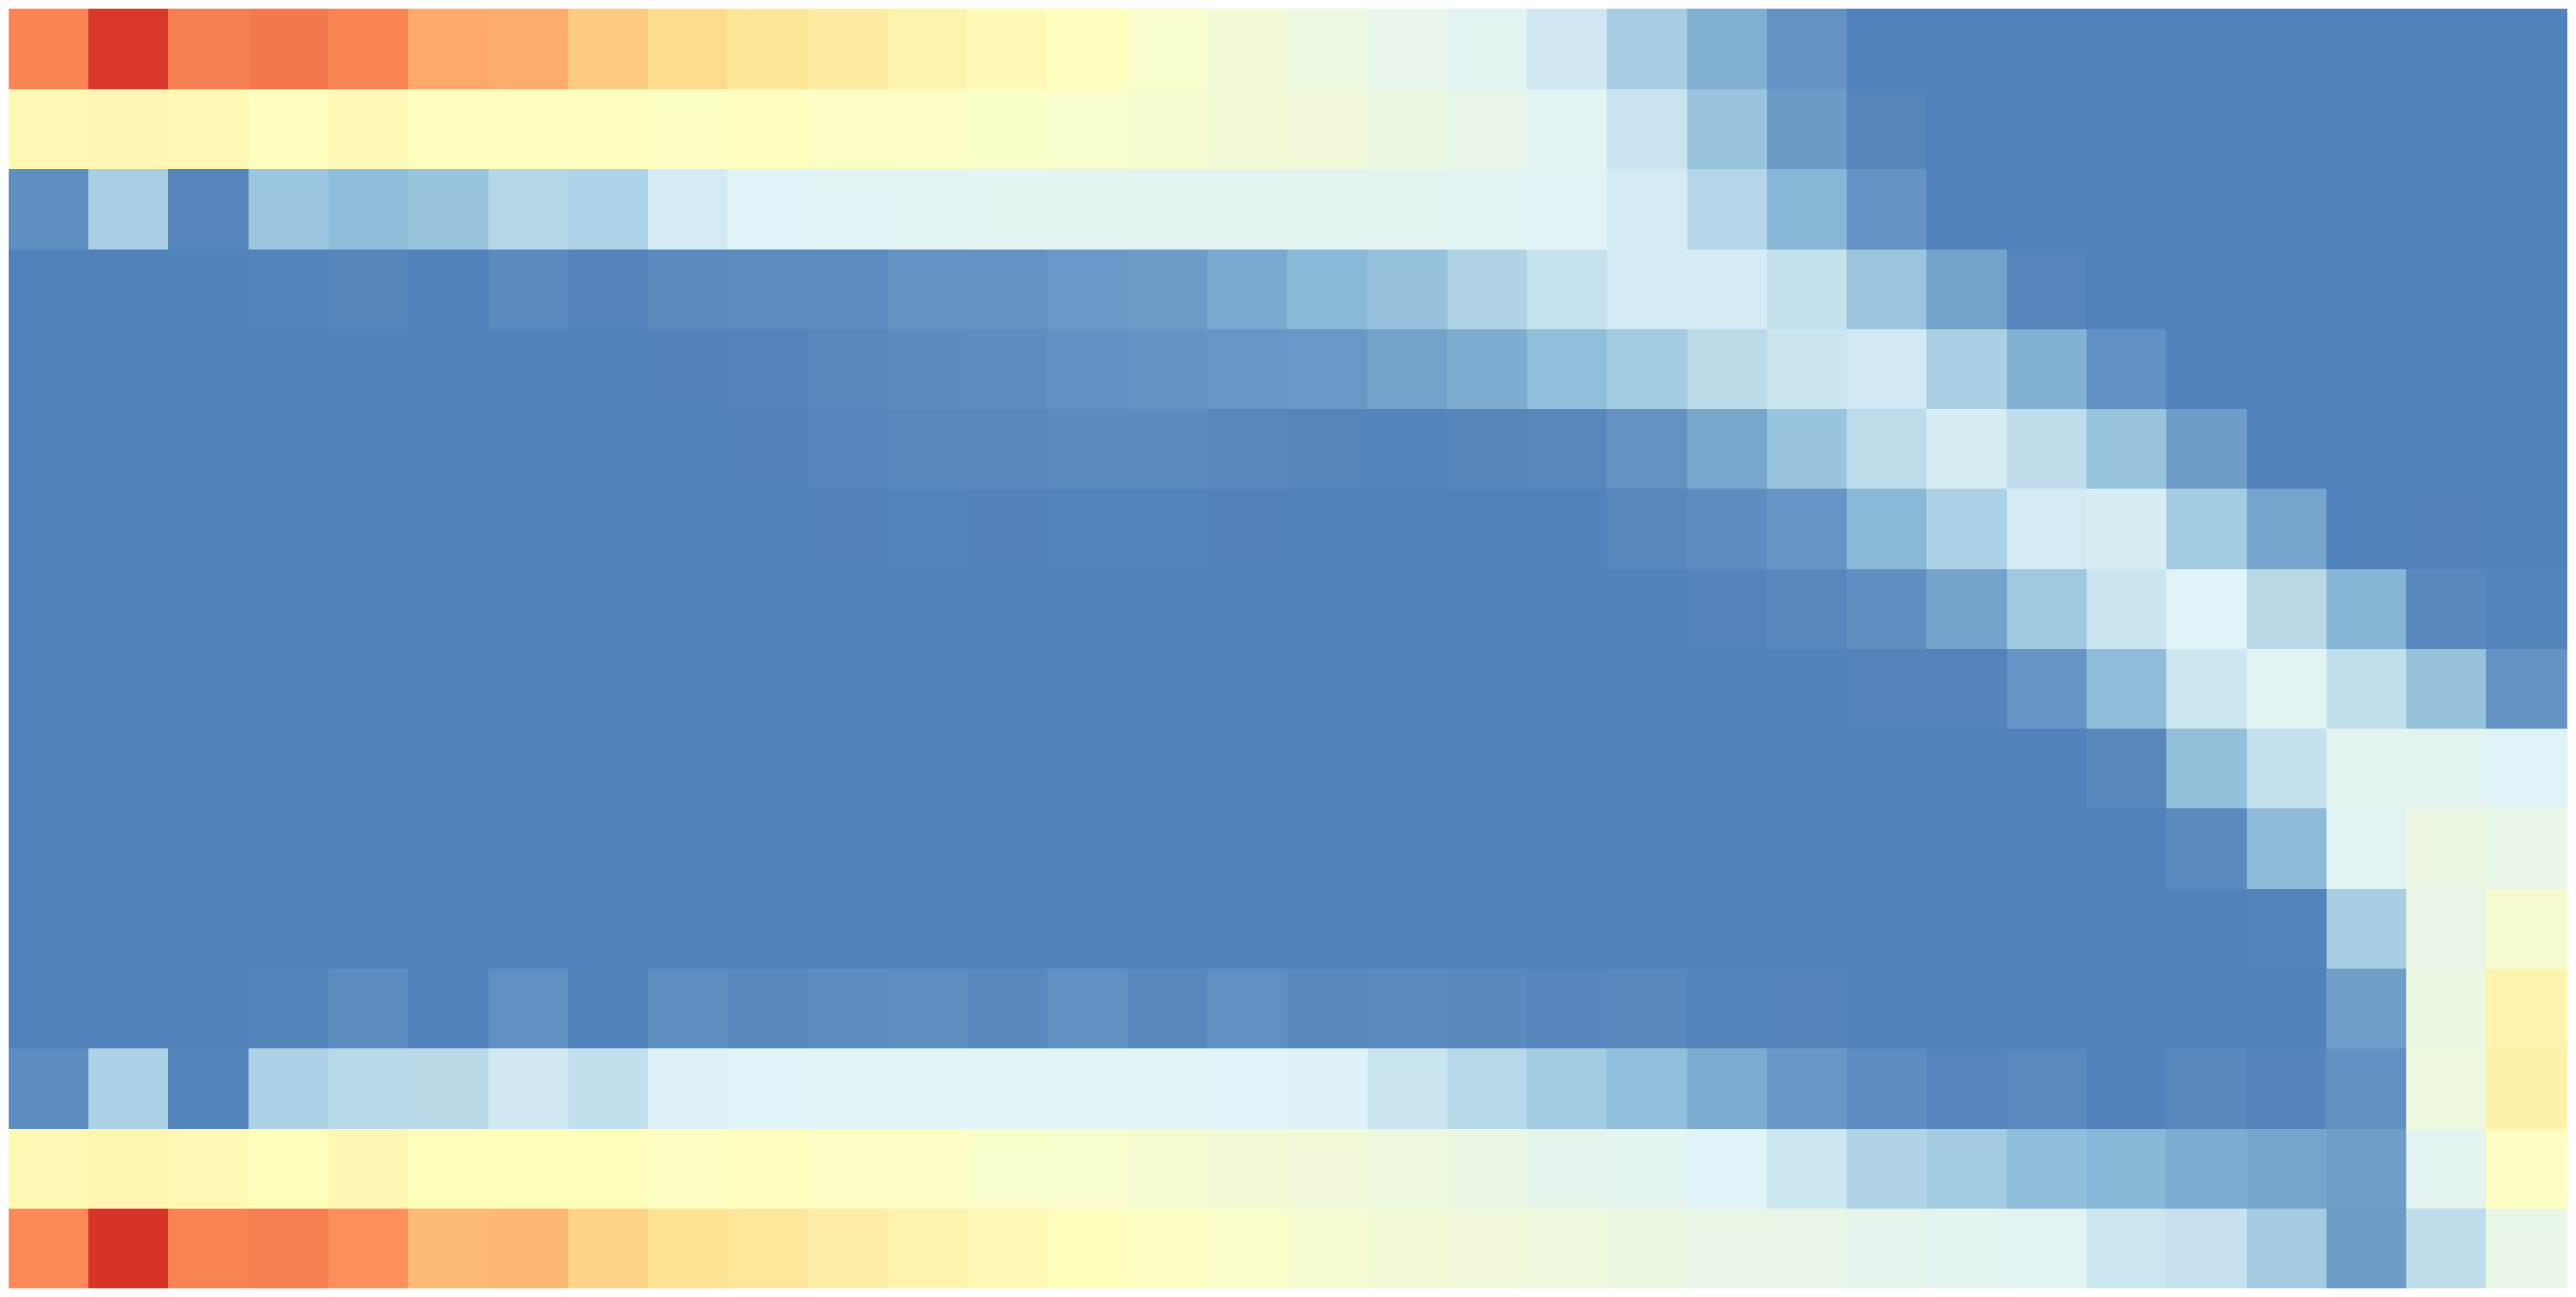
\includegraphics[clip,width=0.5\columnwidth]{./figs/snopt_small.pdf}
% }

\subfloat[Large]{%
  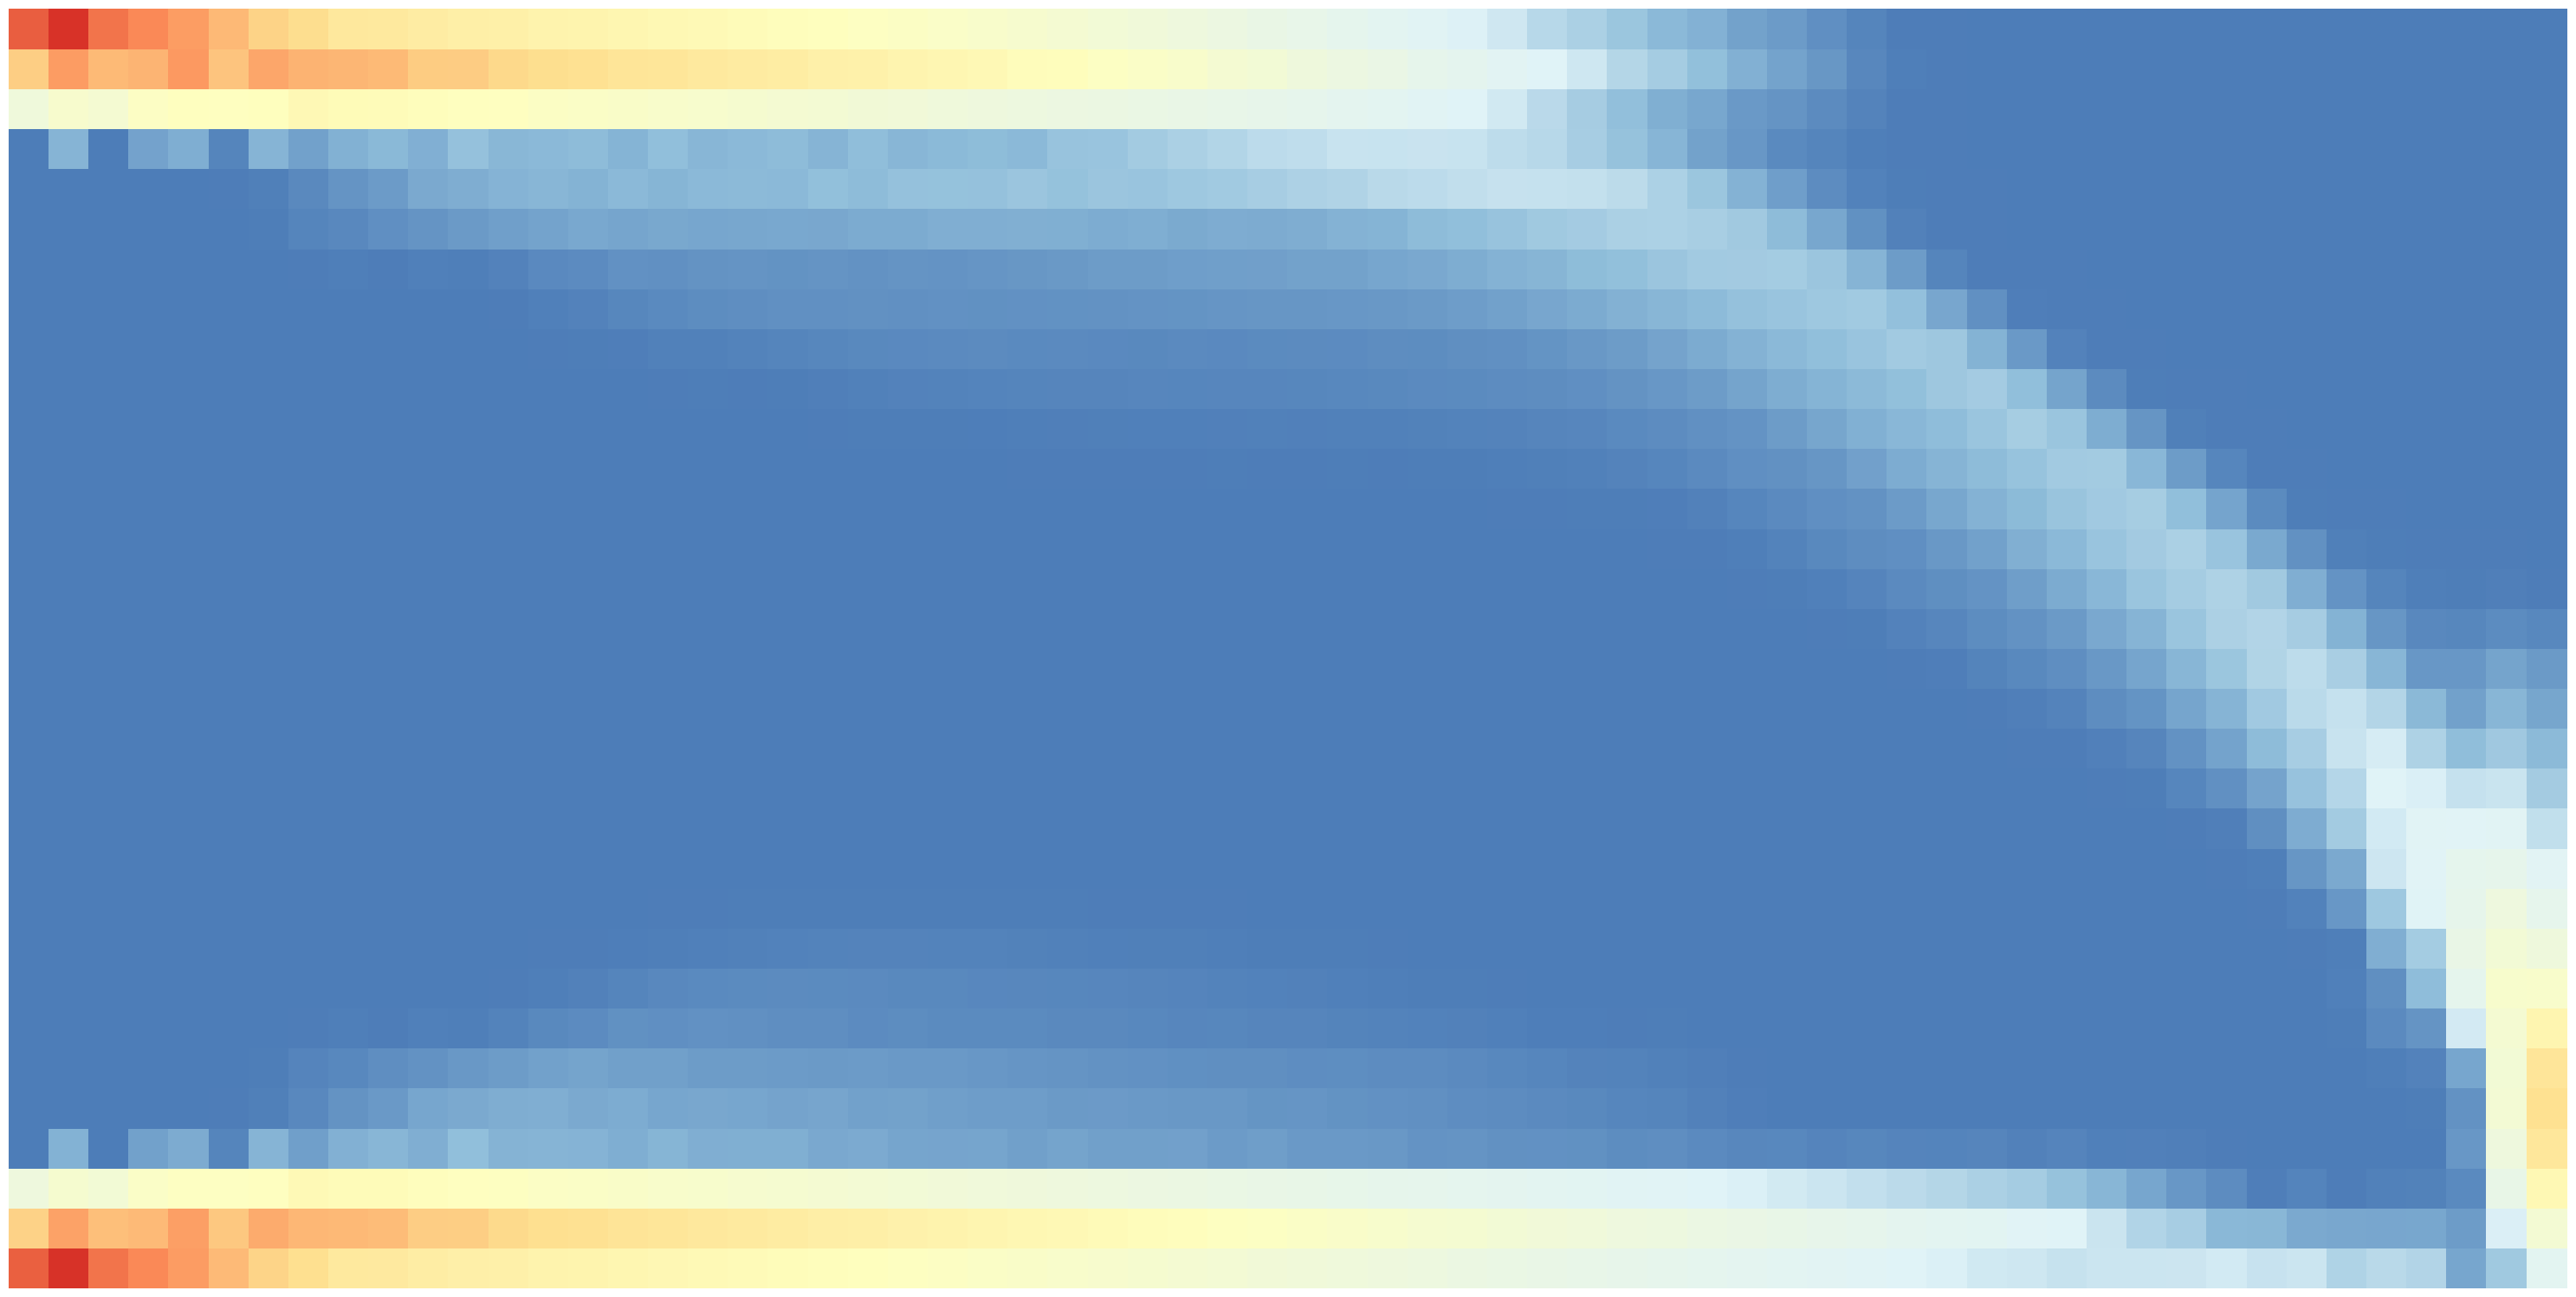
\includegraphics[clip,width=0.8\columnwidth]{./figs/medium2_thick.pdf}%
}
% \subfloat[Medium: SNOPT thickness]{%
%   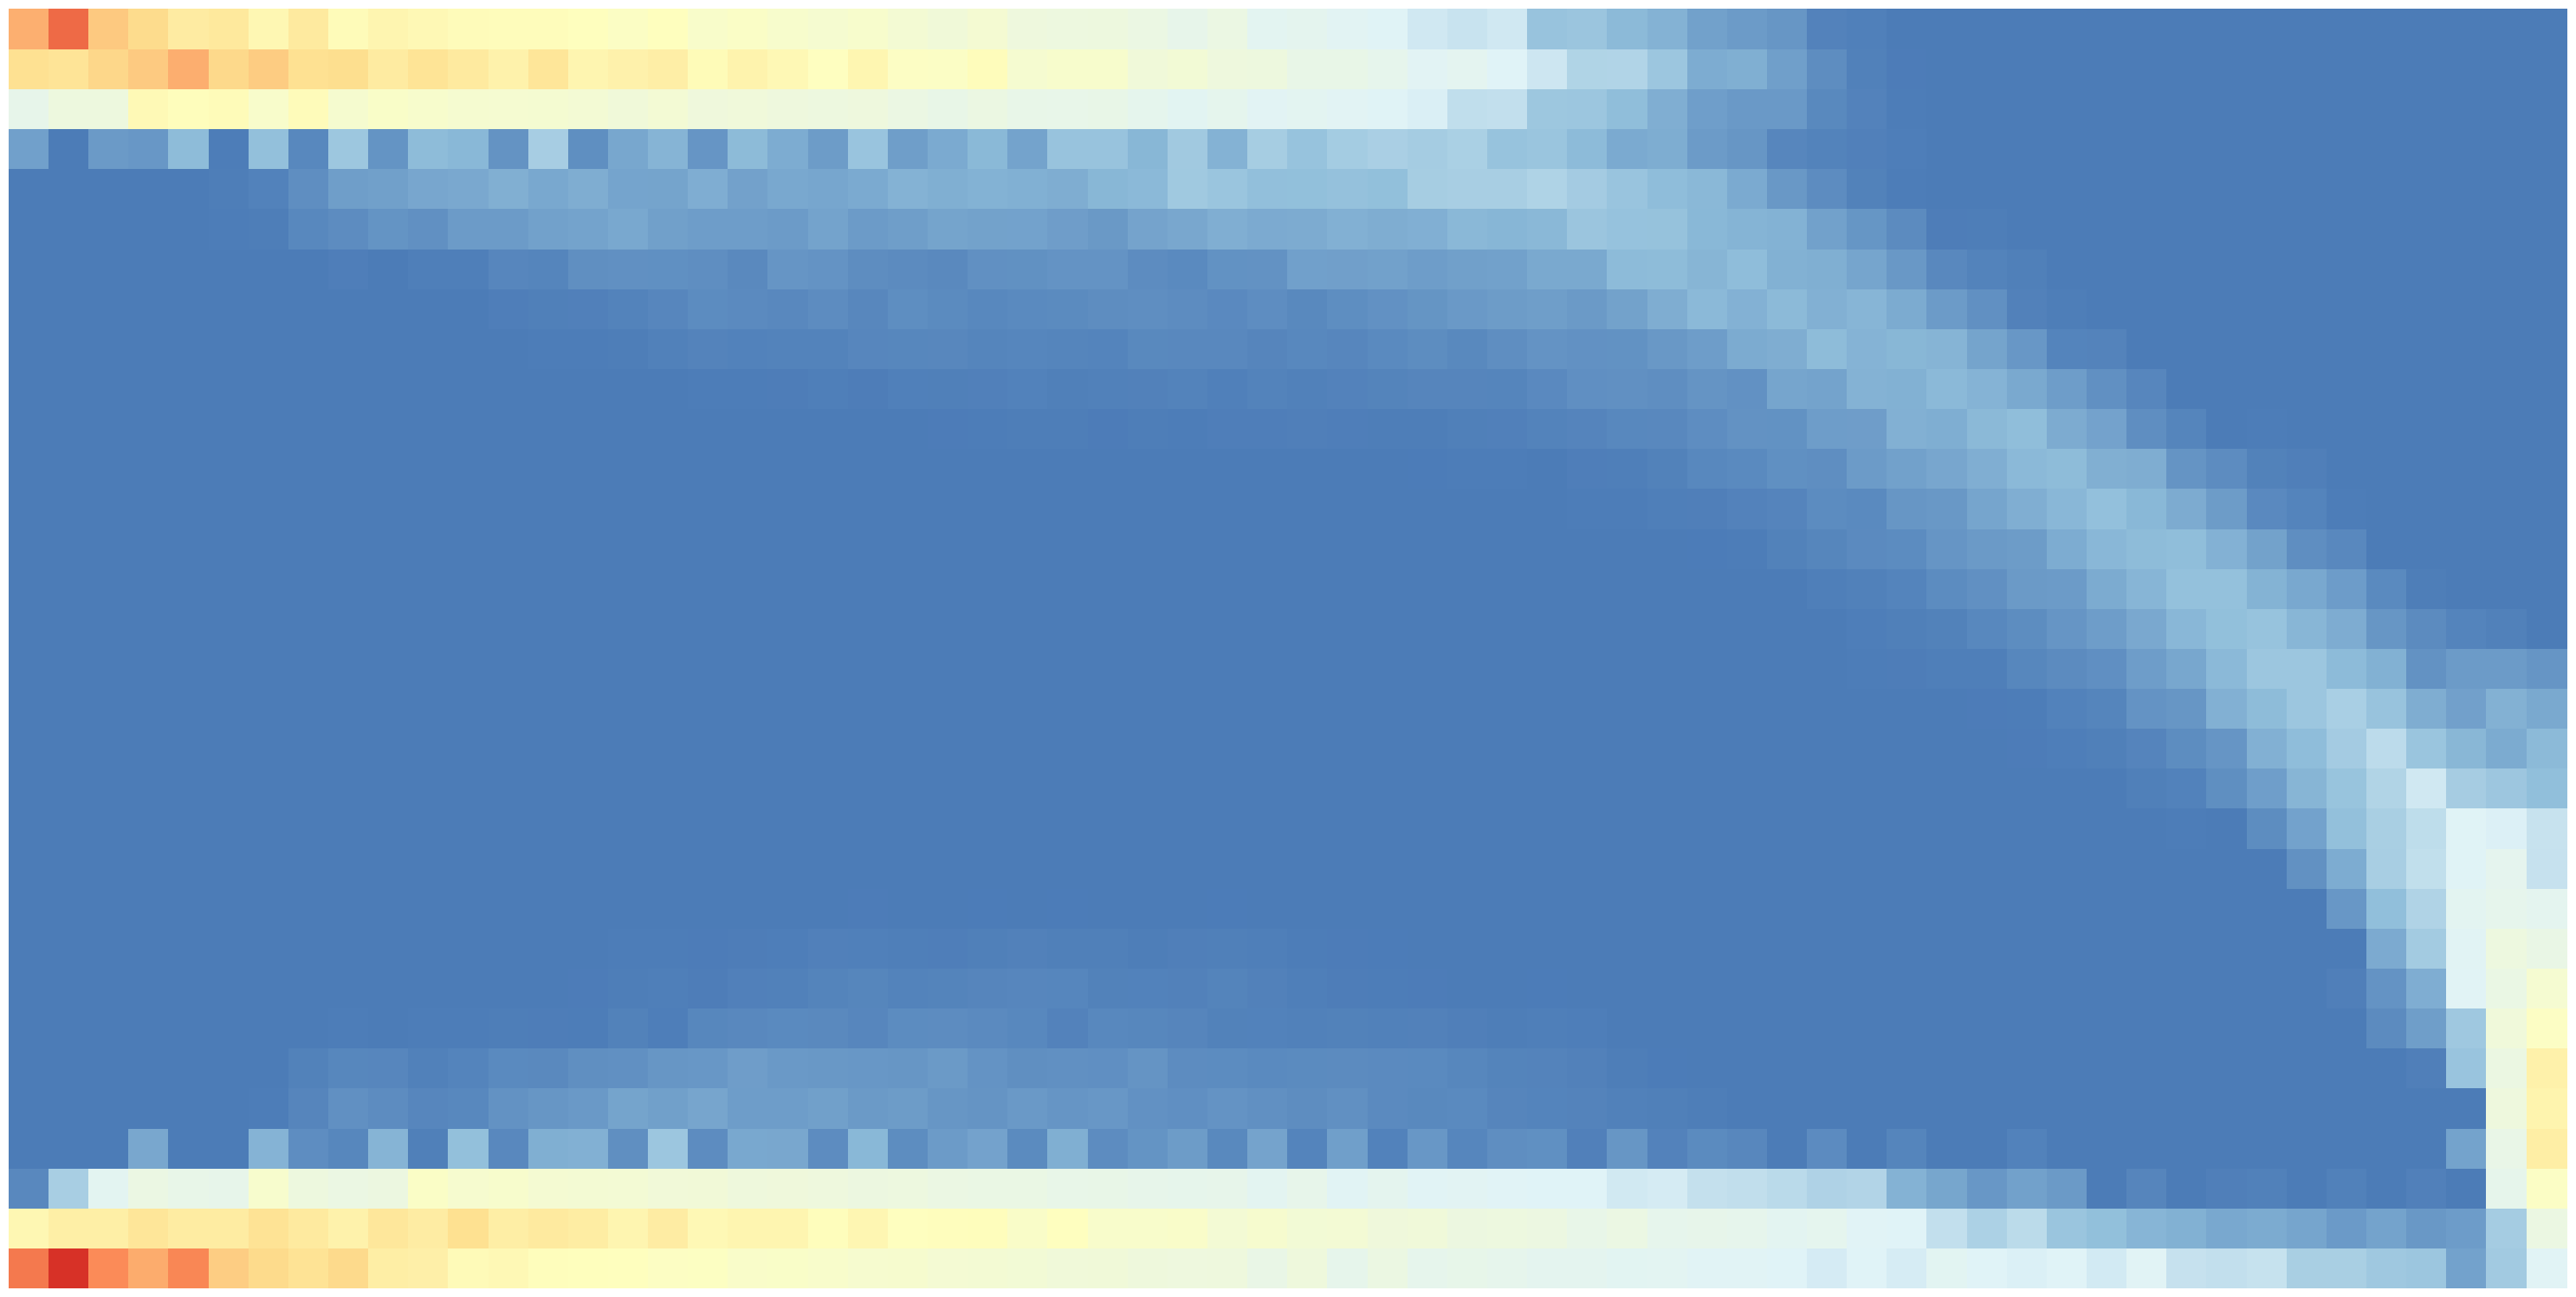
\includegraphics[clip,width=0.5\columnwidth]{./figs/snopt_medium.pdf}%
% }
\caption{Thickness distribution using the new method}
\label{fig:thick}
\end{figure}

\section{Conclusions and Future Work}
In this work, a matrix-free optimization algorithm for reduced-space PDE-constrained problems is developed, where nonconvexity and complementarily are handled using a homotopy map and predictor-corrector method. A novel and effective matrix-free preconditioner has been created for accelerating the convergence rate of the iterative solver. The optimization method itself can handle both equality and inequality constraints, but the preconditioner is designed only for inequality constraints at present. 

The optimization algorithm is based on the homotopy continuation method that constructs a homotopy map of the nonlinear KKT system of equations with a simple linear system of equations. A predictor-corrector algorithm is used to trace the solution curve of the homotopy map as the continuation parameter changes from $1.0$ to $0.0$. The predictor iteration is comprised of a single linear system solver and updates the solution point and continuation parameter simultaneously; the corrector iteration is comprised of a Newton-Krylov module that brings the predictor point closer to the zero path of the homotopy map with the continuation parameter fixed. The kernels of the predictor and corrector iterations are consisted of solutions to two linear systems, with the Jacobian of the Homotopy map being the system matrix for both and different right-hand-side vectors. The two linear systems are solved by a Krylov iterative method that only needs the matrix-vector products of the Homotopy Jacobian matrix with an incoming vector, and the matrix-vector products are calculated matrix-freely using second-order adjoints. 

Based on the results of the test problems, the proposed optimization method can successfully solve the general equality and inequality constrained problems governed by PDE systems. It can handle a moderate amount of nonconvexity in the Hessian of the Lagrangian. The proposed matrix-free preconditioner is effective for the constructed quadratic problem as well as the structural sizing design problem. 

Future work will focus on improving the robustness of the proposed optimization method in the context of nonconvex problems, extending the preconditioner to include equality constraints, and exercising the new method on a benchmark Aerodynamic Shape Optimization problem. 

\newpage

\bibliographystyle{plain}
\bibliography{jehicken.bib} 


%%%%%%%%%%%-----  Homotopy Interior Point --------%%%%%%%%%%%
%In order to describe the homotopy method, we reformulate \eqref{eq:redform} using slack variables:
%\begin{equation}\label{eq:4}
%\begin{aligned}
%&\text{min}   &f(x) &\\
%&\text{s.t.} &  h(x) &= 0 \\
%& &  g(x) - s &= 0 \\
%& &        s  &\geq 0 
%\end{aligned}
%\end{equation}
%where $s \in \mathbb{R}^{m}$ is a vector of slack variables and we have dropped the dependence on $u(x)$ to simplify the presentation.

%The \textit{Karush-Kuhn-Tucker} (KKT) conditions, that is, the first-order necessary optimality conditions at the solution of \eqref{eq:4} are
%\begin{equation}\label{eq:opt0}
%\begin{aligned}
%\nabla f(x) + \lambda_h^T \nabla h(x) + \lambda_g^T \nabla g(x) &= 0, \\
%-\mathcal{S} \Lambda_g e &= 0,\\
%h(x) &= 0, \\
%g(x) - s &= 0, \\
%s \geq 0, \quad &\lambda_g \leq 0. \\
%\end{aligned}
%\end{equation}
%One of the difficulties in solving \eqref{eq:opt0}, in contrast with the PDEs in simulation systems, lies in the sign requirement for the slacks and Lagrangian multipliers. In the optimization process, the slacks have to be non-negative to guarantee feasibility of the inequality constraints, and the multipliers have to be non-positive at a local minimizer. Respecting the bounds during the optimization process can help it converge to a true solution, rather than a spurious solution of the KKT system. At a solution, for each inequality constraint, either the slack or Lagrangian multiplier is strictly zero under the strict complementarity assumption, which basically says the inequality constraints should be clearly either active or inactive at the solution. Active inequality constraints have zero-valued slack variables and negative multipliers in our way of formulation, while inactive inequality constraints have positive slack variables and zero-valued multipliers.
%
%One type of the popular interior-point methods \cite{Nocedal2006NO} deserves being briefly mentioned here due to its close proximity with this research; the Newton-Lagrangian line-search interior-point method. In the continuation approach, a series of perturbed KKT systems are solved for a series of continuation parameter $\mu$ which represents the perturbation amount and goes to zero in the end:  
%\begin{equation}\label{eq:kkt1}
%\begin{aligned}
%\nabla f(x) + \lambda_h^T \nabla h(x) + \lambda_g^T \nabla g(x) &= 0 \\
%-\mathcal{S} \Lambda_g e - \mu e &= 0\\
%h(x) &= 0 \\
%g(x) - s &= 0 \\
%s \geq 0, \quad &\lambda_g \leq 0 \\
%\end{aligned}
%\end{equation}
%where $\mathcal{S}$ and $\Lambda_g$ are diagonal matrices with the slacks and the inequality multipliers on the diagonal respectively, $e$ is a vector of ones in proper dimension. 
%
%At each value of $\mu$, the nonlinear system of \eqref{eq:kkt1} is usually solved by SQP method with direct linear solvers \cite{Byrd:1999:IPA:588897.589167}. The solution trajectory converges to the KKT point of the original problem in the limit as $\mu \rightarrow 0$. 
%
%Several critical and sensitive issues need careful treatment for a successful solution \cite{Nocedal2006NO}. The continuation parameter $\mu$ in Equation \eqref{eq:kkt1} is in place for addressing the nonlinear complimentarity condition, not convexity. Additional globalization methods are needed using either a merit function or a filter to select quality steps that guarantee smooth progress towards the solution. Also in needed are an efficient updating strategy for $\mu$ that decreases neither too slow nor too fast on the way to zero, and a proper amount of regularization to handle nonconvexity and singularity that guarantees the resulting step update is a descent direction. 
%
%In comparison, we have found that the proposed homotopy-based optimization method is advantageous, because it simultaneously addresses nonconvexity, complimentarity, and ill-conditioning of the KKT matrix at intermediate iterates in matrix-free ways. In contrast, most interior point algorithms use direct linear algebra solvers based on factorization of explicit matrices to solve the subproblems. Although inexact variations exist \cite{Gondzio2012}, both the method and the preconditioners used are quite sophisticated with many parameters.
%
%

%-----------------------------------------------------%
% backup slides: on Preconditioner system with \mu = 0.0
% Then we repeat the process of first reducing the system \eqref{eq:pcwithmu} by eliminating the slack and inequality multipliers row block, applying the Sherman-Morrison and truncated SVD approximation to the reduced system in design, and finally retrieving the slack and inequality multiplier updates.  

% The preconditioning system that approximates the KKT system is as follows, without considering the homotopy term:
% \begin{equation}\label{eq:preconditioner2}
% \begin{bmatrix} \tilde{\mathcal{W}} & 0 & \tilde{\mathcal{A}}_{h}^T & \tilde{\mathcal{A}}_{g}^T \\
% 0 & -\Lambda_g \mathcal{S}  & 0 & -\mathcal{S} \\
% \tilde{\mathcal{A}}_{h} & 0 & 0 & 0 \\
% \tilde{\mathcal{A}}_{g} & -\mathcal{S} & 0 & 0
% \end{bmatrix}\begin{bmatrix} v_x \\ v_s \\ v_h \\ v_g \end{bmatrix}=\begin{bmatrix} u_x \\ u_s \\ u_h \\ u_g \end{bmatrix},
% \end{equation}
% where $\tilde{\mathcal{A}}_{h}$ and $\tilde{\mathcal{A}}_{g}$ are approximations to the equality and inequality constraint Jacobians. Next eliminate the slack and inequality multiplier row blocks to get
% \begin{equation}\label{eq:reducedX2}
% \begin{bmatrix} \tilde{\mathcal{W}} +  \tilde{\mathcal{A}}_{g} ^T\Sigma \tilde{\mathcal{A}}_{g} &  \tilde{\mathcal{A}}_{h}^T \\
% \tilde{\mathcal{A}}_{h}  & 0 
% \end{bmatrix}\begin{bmatrix} v_x \\ v_h  \end{bmatrix}=\begin{bmatrix} u_x- \tilde{\mathcal{A}}_{g}^T \Sigma(-u_g + \Lambda_g^{-1}u_s  )  \\ u_h \end{bmatrix},
% \end{equation}
% where $\Sigma = -\mathcal{S}^{-1} \Lambda_g $. After computing $v_x$ and $v_h$,  $v_g$ and $v_s$ can be obtained from the equations:
% \begin{equation}\label{eq:vgvsnomu}
% \begin{aligned}
% v_g & = \Sigma(-u_g + \Lambda_g^{-1}u_s  + \tilde{\mathcal{A}}_{g} v_x)   \\
% v_s &= -\Lambda_g^{-1}  v_g -  \Lambda_g^{-1} \mathcal{S}^{-1} u_s
% \end{aligned}
% \end{equation}

% We need an inexact solution to \eqref{eq:reducedX2}. An approximate solution is sufficient, since our present goal is an efficient preconditioner.  However, the inexact solution method must be inexpensive and matrix-free.  To this end, we begin by replacing $\tilde{\mathcal{W}}$ with a diagonal matrix. For inequality-constrained problems, the system \eqref{eq:reducedX2} becomes:
% \begin{equation}\label{eq:focusX}
% (\tilde{\mathcal{W}} +  \tilde{\mathcal{A}}_{g} ^T\Sigma \tilde{\mathcal{A}}_{g} ) v_x = u_x- \tilde{\mathcal{A}}_{g}^T \Sigma(-u_g + \Lambda_g^{-1}u_s  ) 
% \end{equation}

% For the term $\tilde{\mathcal{A}}_{g} ^T\Sigma \tilde{\mathcal{A}}_{g}$, we have the matrix-vector products available, but not the explicit matrices. Therefore, we apply the Lanczos algorithm using matrix-vector products based on $\tilde{\mathcal{A}}_{g} ^T\Sigma \tilde{\mathcal{A}}_{g}$ to make a low-rank truncated SVD approximation. 
% \begin{equation}
% \tilde{\mathcal{A}}_{g} ^T\Sigma \tilde{\mathcal{A}}_{g} = M_{m\times k}\Gamma_{k\times k} N^{\star}_{k\times m}
% \end{equation}
% where the columns of $M$ are the left-singular vectors, the diagonal elements of $\Gamma$ are the singular values, and the columns of $N$ are the right-singular vectors.   

% Next,  we use the generalized Sherman-Morrison equation to get the direct inverse of $\tilde{\mathcal{W}} +  \tilde{\mathcal{A}}_{g} ^T\Sigma \tilde{\mathcal{A}}_{g} $. Recall that the generalized Sherman-Morrison is as follows: 
% \begin{equation}\label{eq:sherman}
% \begin{aligned}
% B &= A + UV \\
% B^{-1} &= A^{-1} - A^{-1}U(I_k + VA^{-1}U)^{-1}VA^{-1} 
% \end{aligned}
% \end{equation}
% where $A$ is a square invertible $n\times n$ matrix,  $U$ is $n \times k$ matrix and  $V$ is $k\times n$ matrix, and it is assumed that $( I_k + VA^{-1}U )$ is invertible. 

% Comparing \eqref{eq:sherman} and \eqref{eq:focusX}, we make the associations
% \begin{equation}\label{eq:sherman_svd2}
% \begin{aligned}
% B  &=  \tilde{\mathcal{W}} +  \tilde{\mathcal{A}}_{g} ^T\Sigma \tilde{\mathcal{A}}_{g}, \\
% A  &=  \tilde{\mathcal{W}}, \\
% U  &= M_{m\times k},    \\
% V  &=  \Gamma_{k\times k}N^{\star}_{k\times m}. 
% \end{aligned}
% \end{equation} 

% Therefore:
% \begin{equation}\label{eq:sm_svd3}
% \left(\tilde{\mathcal{W}} +  \tilde{\mathcal{A}}_{g} ^T\Sigma \tilde{\mathcal{A}}_{g}\right)^{-1} = \tilde{\mathcal{W}}^{-1} - \tilde{\mathcal{W}}^{-1} M \left( I_k +\Gamma N^{\star}  \tilde{\mathcal{W}}^{-1} M \right)^{-1} \Gamma N^{\star} \tilde{\mathcal{W}}^{-1}  
% \end{equation}

% From here, we first calculate the right-hand-side of \eqref{eq:focusX}, then multiply it with \eqref{eq:sm_svd3} to get the preconditioned design update. The preconditioned inequality multiplier and slack update are computed using \eqref{eq:vgvsnomu}.   
\end{document}
